\documentclass{article}
\usepackage{hyperref}
\usepackage{float}
\usepackage{csquotes}
\usepackage[style=iso]{datetime2}
\usepackage[usenames,dvipsnames]{color}
\usepackage{booktabs}
  \setlength\heavyrulewidth{0.20ex}
  \setlength\cmidrulewidth{0.10ex}
  \setlength\lightrulewidth{0.10ex}

\usepackage[font=normalsize,labelfont={bf}]{caption}
  \captionsetup[table]{aboveskip=3pt}

\hypersetup{
    colorlinks=true,
    linkcolor=blue,
    filecolor=magenta,      
    urlcolor=magenta,
 }
 
\usepackage{graphicx}
\graphicspath{ {./img/} }
\renewcommand{\abstractname}{DISCLAIMER}
\title{A PRACTICAL GUIDE TO FEMINIZING HRT}
\author{\href{https://katea.gay/}{Katie Tightpussy}}
\date{\today}
\setcounter{section}{-1}
\urlstyle{same}

\begin{document}


\maketitle
\tableofcontents
\begin{abstract}
    I am not a doctor. I do not work in medicine. I am not a medical professional in any capacity. I am a layperson offering lay opinions based on the extent of my own education and experiences. All information and assertions below should be treated accordingly as mere opinion rather than statement of fact or medical advice. This guide prioritizes community moral truth where scientific research falters. Basically, don’t get mad at me. 
\end{abstract}


\section{FOREWORD}

The purpose of this living document is to catalogue my thoughts and opinions regarding feminizing HRT because I believe that the various community wikis are impractical. They are valuable resources, but in my view these wikis lack utility for people who are more interested in clear actionable guidance than they are in learning every semi-relevant biological progress and graph. I aim to provide an exhaustive quick reference guide of simplified direct answers to the most common questions on how to safely and effectively perform HRT that I have received over the years with the goal of demystifying this life saving medicine both for people considering HRT and for established transsexuals. As such, I assume a baseline familiarity with the effects of HRT. In case you are not familiar: HRT does a lot and probably more than you think. It’s great. \textbf{Changing your sex is really cool and fun. I recommend it.} You deserve quality transition healthcare and are capable of making the best decisions for yourself. I hope that this document can be a useful tool in your decision-making process and a starting point for further learning if that is your interest.

And stay off the trans subreddits, too. Just trust me on that one, okay? Or at the very least /r/mtf since that one is particularly bad. Neither healthy places nor sources of good wisdom. You’ll be pulling rotten brain worms out for years. Best advice I can give.

As for the fellas, sections of this are still highly relevant, but obviously there are key differences in goals and outcomes. \href{https://docs.google.com/document/d/1DXFxzN0XTudPZez\_SO61fpqncRLPH\_Be\_QG\_8Pcz9LU/edit?tab=t.0}{This guide for masculinizing HRT} \textcolor{red}{(Warning: Google Docs link)} looks pretty solid, but I haven’t examined it in full depth, so use your brain and your judgement. Anyway they should make a tboy Katie Tightpussy. Oliver Longdick or something. Maybe Xavier.

\textbf{If you would like to donate to support this project,} \href{https://cash.app/Katitties}{CashApp}, \href{https://ko-fi.com/katitties}{Ko-Fi}, and \href{https://account.venmo.com/u/katitties}{Venmo} all work. I appreciate it!

\subsection*{How to Use This Document}

This document is structured linearly as a series of questions and answers such that broadly-speaking each question and section flows into the next. I encourage reading it top-to-bottom as that should hopefully answer any questions (including ones you didn’t know that you had) in a conversational narrative, but obviously this is lengthy. Take your time and read it in pieces if you wish.

You can use the table of contents to navigate to a particular section or question as needed, especially when re-visiting. I recommend saving this page / document so that you can refer back to it any time you have questions about your HRT. It is a lot to absorb up front, so it’s okay if it doesn’t! No rush on any of this.

\noindent\textbf{\href{pghrt.pdf}{This document can also be downloaded as a PDF. Please do so.}}

\noindent\href{pghrtgretchensversion.txt}{Alternatively, you can read a 90s-00s style .txt version if you are inclined.} It won't stay up to date though.

\noindent\textbf{If you are interested in doing a translation or any other alternate version, please get in touch!}



\section*{DEDICATION}
\addcontentsline{toc}{section}{DEDICATION}

This document is dedicated to all of our sisters who did not make it. May we carry the light of their torch into another day.

 

\section{INTRODUCTION}

\subsection{Is taking estrogen safe?}

With modern bioidentical hormones, HRT could not be much safer. You’re just flipping the primary juice that your body runs on and shifting the balance of hormones that are already in your body. Even where the details of optimization get complex, the core principle of changing your biology is highly forgiving. The body is malleable and you will be able to adjust to what feels right for you.

\subsection{What route of administration should I choose for estrogen?}

Injections. They are on the whole the most effective, easy, consistent, safe, and inexpensive form of HRT. For some, injections become a ritual to look forward to, and others they can become quite fun.

\noindent\underline{\textbf{But remember: any estrogen is better than no estrogen.}}

\subsection{Why do you not recommend pills, patches, or gel?}

Chiefly, all three have major downsides that injections do not. It is not that they do not work, it is that you deserve better than being forced to tolerate major downsides. Let me reiterate: \textbf{all forms of HRT can produce satisfactory results}, but that does not mean all forms of HRT are equal or good.

\subsection{Is dosage of estrogen equivalent across administration routes or forms?}

No. This is important enough that I did not relegate it to Section \ref{MM} “MYTHS AND MISCS”. \textbf{Estrogen dosages cannot be directly compared across type or form.} 1mg of one is not 1mg of another. Different types and forms have different properties that affect how much estrogen is absorbed into the body (\textit{“bioavailability”}), at what rate, and the resulting half-life.

\subsection{What is a “half-life”?}

In simple terms, the \textit{half-life} of a substance is the time it takes until half of that substance is eliminated. In the context of HRT, this is what determines how long a dosage stays active in your system, and thus your dosing frequency. This is referred to as your hormone cycle, and it forms a curve. Levels go up, they peak, and then they fall. The properties of this curve (how estrogen levels change over time) are important.

\subsection{What’s wrong with pills?}

The largest issue with pills is that they carry increased long term blood clotting and liver coagulation risks. The severity of these risks can be mitigated in part by taking them sublingually or buccally (dissolving the pill either underneath your tongue or between your gum and cheek, respectively) as opposed to orally (swallowing the pill normally) to avoid first-pass metabolism in the liver. Even with sublingual and buccal methods, however, it's common to ingest some amount of the pill, so it’s fair to assume that at least some risk remains. Please understand that the absolute risk is still low (e.g., \textit{acetaminophen} has an order of magnitude more liver concerns than estrogen), however \textbf{this risk compounds even further with nicotine-related estrogen risk.} See Question \ref{11-2} as well.

Beyond this, numerous other issues with pills stem from two main characteristics: 1) their short half-life and poor bioavailability, and 2) their common necessitation of antiandrogens. The former characteristic makes pills largely unsuitable for monotherapy (discussed below) when compared to injections. The latter often comes with an assortment of negative side effects depending on the antiandrogens involved (see Section \ref{AA} “ANTIANDROGENS”). Together, these characteristics add additional degrees of variability that make poor regimens and their side effects (such as poor energy/libido and slower results) more common than with other administration routes. Pills are also more difficult to stockpile, and in some marketplaces are more expensive than vials. Please also note that importing pills from foreign distributors in large volumes may run afoul of customs which may lead to seizure, financial loss, and/or possible legal trouble depending on your country's laws. \textbf{If anyone asks, you don't know who ordered those pills.}

\textbf{If you are on pills for whatever reason, please take 4-8mg sublingually spaced throughout the day.} Under 4mg is almost never a sufficient dosage.

\subsection{What’s wrong with patches?}

\begin{itemize}
  \item Relatively expensive (typically even more than pills);
  \item More difficult to procure DIY (only via grey market means);
  \item Generally necessitate an antiandrogen (see Section \ref{AA} “ANTIANDROGENS”);
  \item Can result in skin irritation;
  \item Require being applied 24/7;
  \item Are prone to falling off;
  \item Aren’t always consistent in their absorption (such as with heat);
  \item Are harder to stockpile (difficult to acquire in bulk);
  \item Often fail to exceed menopause levels even with multiple on at once.
\end{itemize}

\subsection{What’s wrong with gel?}

\begin{itemize}
  \item Difficult to dose accurately which leads to inconsistent levels;
  \item Requires regular application of goop due to a relatively short half-life;
  \item Can be messy (goopy);
  \item Risk second-hand exposure via contact with others
  \item Generally necessitates an antiandrogen (see Section \ref{AA} “ANTIANDROGENS”).
\end{itemize}

It should be noted however that gel requires minimal supplies for self-production which is a boon in some circumstances.

\subsection{What about pellets?}

\begin{itemize}
  \item Generally far more expensive than any other option;
  \item Few providers who offer them;
  \item Dosing adjustment periods are highly spread out;
  \item Defective pellets can cause insufficient levels;
  \item Crushed/broken pellets can cause unexpectedly high levels;
  \item Generally not possible to DIY them.
\end{itemize}

The last point in particular means that you can only go to those few likely-expensive providers. It’s possible that this is the first time you have even heard of pellets. See the issue?

\subsection{What about sprays?}

These are still fairly experimental so there is little to say about them, but they share pros and cons with gel. I mostly note this here so that you are aware that they exist.

\subsection{Is the difference that significant?}

\textbf{Yes.} To the point that I wrote all of this so that I could repeat myself less by instead linking this. A properly dosed injection regimen is the best form of estrogen that we have for achieving monotherapy target levels.

 

\section{WHY INJECTIONS}

\subsection{What makes injections so good?}

Consistency. Consistency is the name of the game when it comes to HRT. Consistent hormones means stability, and stability is good. Even the “worst” injection type (keep reading) can provide a more consistent hormonal cycle than other routes of administration which provides many benefits.

\subsection{Are antiandrogens necessary with injections?}

Generally, no. A properly dosed and spaced injection cycle that provides consistently high enough estrogen levels can naturally stop testosterone production which forgoes the need for an antiandrogen which is preferable in most cases. This is referred to as \textit{“monotherapy”}.

\subsection{How does monotherapy work?}\label{2-3}

In simple terms, the brain does not care which hormone it has, just as long as it has enough. If there are consistently enough hormones in your body, it stops producing more. The “consistent” part is what injections are capable of that other administration routes struggle with. Trying to do sufficient monotherapy on pills, for instance, is very likely impossible in most situations. In more specific terms regarding the HPG axis, \textit{luteinizing hormone} (LH) and \textit{follicle-stimulating hormone} (FSH) are suppressed by increased serum \textit{estradiol} levels, thus inhibiting GnRH production and by extension testosterone production in the testes.

\subsection{How are injections safer?}

By generally not necessitating antiandrogens (see Section \ref{AA} “ANTIANDROGENS”), the long term risks associated with antiandrogens are obviated. Bioidentical estrogen that bypasses the liver (see Question \ref{11-1}) is as close as we can possibly get to natural estrogen production which removes additional risk.

\subsection{But aren’t there risks with the physical act of injecting?}

Yes, but with minimal training required (see Section \ref{ts} “TECHNIQUE AND SUPPLIES”), at worst one may experience a minor bruise. It is akin to riding a bike in that once you know how to do it, you would have to try VERY hard to do it significantly wrong.

\subsection{How are injections easier?}

Once you are dialed in, you are good. Injections don’t require frequent administration (e.g., a weekly injection vs multiple daily pills), are not at major risk of inaccurate dosing, cannot fall off mid cycle, and don’t require potentially significant travel to a provider.

\subsection{How are injections cheap?}

In simple terms, far less estrogen is needed. A 5ml vial that is capable of providing nearly a years’ worth of estrogen has only 200mg of estrogen in that vial, whereas a minimum equivalent supply of pills for example (4mg * 365 days = 1460 mg) is substantially more. This is not a rigorous comparison, but it’s a useful demonstration of scale. Another fun comparison is that you can fit 1-2 years of estrogen vials inside of a typical three-month supply bottle of pills.

\subsection{But I don’t have insurance / my insurance won’t cover it / pills are cheaper than injections with my insurance / injections are not available in my country / my doctor won’t prescribe injections?}

Please see Section \ref{sv} “SOURCING VIALS”. You will be amazed, and quite likely, radicalized.

\subsection{Is swapping to injections good even after years on HRT?}

\textbf{Yes.} Nothing is guaranteed, but many people experience substantial noticeable differences after swapping to injections even after years on HRT. These range from increased breast development, improved mental health, alleviated side effects of antiandrogens or other forms of estrogen, generally feeling better, etc. Switching is worth it.

\subsection{But injections are scary?}

Yes, they are at first. Nobody likes needles because the body naturally does not want to poke itself, but with proper technique and supplies, it won’t hurt much at all. There are countless cases of people with debilitating needlephobias who now find the experience of injecting to be boring. The fear is normal and common, but it is wholly surmountable and worth overcoming. “Oh, that wasn’t as bad as I thought,” is a very common sentence. As the mantra goes: do it scared. You’ll be okay.

\subsection{Are injections like a blood draw or a vaccine?}

No. Blood draws typically use much larger needles and go into a more sensitive spot while also draining you of blood which is usually unpleasant. Vaccines contain vaccines which cause painful immune reactions because they are vaccines. HRT injections put a small amount of hormones in you which causes you to feel good because you have hormones in you. You see the difference, I trust. The act of injecting yourself can also be easier than someone else injecting you, depending on your inclination.

\subsection{Are there any accessibility tools for injections?}

Yes. Auto-injectors exist and can be quite useful if you have fine motor control issues for instance. Please see Question \ref{5-21}, or just keep reading.

\subsection{But I \textit{am} special and can’t inject because I have glass bones and paper skin and\textemdash{}?}

I understand the fear, but if you truly do not wish to do injections under any circumstances and don’t have some sort of legitimate contraindication like hemophilia, then don’t. You can just say that. It’s fine. When you change your mind, this guide will still be here. And if you don’t, so be it. 

 

\section{TYPES AND DOSAGES}\label{td}

\subsection*{Key Vocabulary}
\addcontentsline{toc}{subsection}{\textemdash{} Key Vocabulary}

\subsection{What are the different types of injectable estrogen?}

The four main types used for HRT are \textit{estradiol valerate} (EV), \textit{estradiol cypionate} (EC), \textit{estradiol enanthate} (EEn), and \textit{estradiol undecylate} (EUn). Each of these is an “ester” of \textit{estradiol} and will be converted to \textit{estradiol} in your body. 

Please note that in some regions pills are confusingly sold with the name \textit{estradiol valerate}, but this section only refers to the injectable form.

\subsection{What are the differences between each type of injectable estrogen?}

The only relevant difference between esters is that each has a different half-life and resultant hormone curve which in turn affects dosage and frequency.

\subsection{Does one type of injectable estrogen feminize better than another?}

\textbf{No.} The differences affect dosage and frequency which is a qualitative difference in experience that can make one ester preferable to another, but all four types work acceptably well and retain the benefits of injections. 

\subsection{What type of injectable estrogen should I choose if I have the choice?}

If you have the choice, \textit{estradiol enanthate} is preferred for most people due to the exceptionally stable levels it provides, with the caveat that in most countries this choice only exists if you are doing DIY (see Section \ref{sv} “SOURCING VIALS”). If you are going through a doctor, you may have the option of \textit{estradiol cypionate}, but usually in low concentrations which can make the benefits moot depending on your tolerance for high volume injections. The most commonly prescribed injectable estrogen (particularly in the US), \textit{estradiol valerate}, is still fully capable of producing good results, but it has some minor annoyances that make it not preferred when there is the choice for otherwise (i.e., when doing DIY). Keep reading.

\subsection{What is “concentration”?}

Estrogen vials are made from estrogen held in an oil solution. The \textit{concentration} of a vial is the amount of estrogen held in that solution. This is given as a ratio of mass to volume for the vial. In other words: for every one milliliter of oil (volume measurement), there is that many milligrams of estrogen (mass measurement). You will often see concentrations listed by the vial’s total volume (e.g., 200mg / 5ml) but it is always preferred to simplify this fraction (so 40 mg/ml in this case). \textbf{Typical concentrations are 5 mg/ml, 10 mg/ml, 20 mg/ml, 40 mg/ml, and occasionally 50 mg/ml.}

\subsection{What is meant by “dosage and frequency”?}

\textit{Dosage} and \textit{frequency} are the two factors that determine your hormone cycle. \textit{Dosage} refers to how much estrogen you put in you (measured in mg), and \textit{frequency} refers to how often you put estrogen in you (measured in days or weeks). You will often hear the word “regimen” as well, referring to everything HRT-related that you are taking and at what frequencies.

\subsection{How do I know what my dosage is?}

Your dosage is the concentration of your vial multiplied by the volume that you are injecting. \[Concentration (mg/ml) * volume (ml) = dosage (mg)\] \textbf{Please understand that volume alone is not a dosage.} An analogy would be with baking: you cannot just say “bake for 45 minutes” because you have to know what temperature to set the oven.

\subsection{What are some example dosage calculations?}

The math is simple, I promise! Below is a small reference table comparing concentrations and volume for a range of common dosages. Stick to only two decimal places. You won’t be using syringes that have the accuracy for a number like 0.153ml for instance. That’s within rounding error and isn’t a relevant difference at our scale.

\begin{table}
\centering
\caption{Example Dosages for Common Concentrations by Volume}
\label{tab:concentrations}
\begin{tabular}{@{}lllll@{}}
    \toprule
    \multicolumn{1}{c}{} & \multicolumn{4}{c}{Concentrations (mg/ml)} \\
    \cmidrule(rl){2-5}
            & 5    & 10  & 20 & 40    \\
            \cmidrule(rl){2-5}
Dosage (mg) & \multicolumn{4}{c}{Volume (mL)}  \\
    \cmidrule(r){1-1} \cmidrule(lr){2-5} 
4        & 0.8  & 0.4 & 0.2  & 0.1      \\
5        & 1    & 0.5 & 0.25 & 0.13   \\
6        & 1.2  & 0.6   & 0.3  & 0.15     \\
7        & 1.4  & 0.7 & 0.35  & 0.18  \\
8        & 1.6  & 0.8   & 0.4  & 0.2    \\
9        & 1.8  & 0.9 & 0.45  & 0.23 \\
10       & 2    & 1   & 0.5  & 0.25   \\
    \bottomrule
\end{tabular}
\end{table}

\textbf{How to read this chart:} Take your desired dosage on the left and find the corresponding volume on the right for your given concentration in the column at the top. You will notice that the volume requirements for 5 mg/ml vials to have reasonable dosages is not good. That is because 5 mg/ml vials are not good. 

\subsection{How do I convert dosages between esters?}

\textbf{You don’t. }Because they behave differently, there isn’t a “conversion” between dosages in that sense. If you swap from one ester to another, you should just do a typical dosage for the new ester and work from there. You can make comparisons between them, but there is no method to convert one to another.

\subsection{How can I compare different curves and dosages between esters?}

If you would like to get nerdy, I rate \href{http://estrannai.se}{estrannai.se} quite highly. Keep in mind that this isn’t required but it is a good tool for performing rough comparisons. \href{https://estrannai.se/\#i0__cu,7,7,1-cu,5,7,3-cu,5,7,2}{Here is an example comparison between typical weekly dosages} which we will now see individually.

\textbf{It should be noted that the dosages I list below should be sufficient on the lower end of the range in most cases.} Start with the lower number and move up if you need. More is not inherently better, but we will discuss that in depth later. These dosage ranges are unlikely to change regardless of where you acquired your vial.

\subsection*{Meet Your Esters}
\addcontentsline{toc}{subsection}{\textemdash{} Meet Your Esters}

\subsection{How do I dose \textit{estradiol valerate}?}

Either twice a week at a lower dosage or once a week at a higher dosage is necessary for good levels with \textit{estradiol valerate}. It is a matter of comfort and tolerance. The typical rule of thumb is about 1mg for every day in a cycle with frequencies generally between 3-7 days. \textbf{A weekly dosage between 6-8mg is my typical recommendation}, but 4-5mg per 5 days is also very common. \textbf{The frequency should never be less often than weekly (i.e., No more than seven days between injections).} Weekly is already pushing how long the ester can last. Anything further is highly discouraged to avoid side effects related to variance (See Question \ref{7-3}).

Please note that in some regions pills are confusingly sold with the name \textit{estradiol valerate}, but this section only refers to the injectable form.

\subsection{How is the hormone curve for \textit{estradiol valerate} characterized?}

\textit{Estradiol valerate} is the most finicky of esters. It rapidly spikes to a very high peak a few days after injection and just as quickly crashes back down. This relative instability can be unpleasant depending on your personal sensitivities, but with adjustments to frequency and dosage this can be mitigated to a degree.

 \begin{figure}[H]
     \centering
     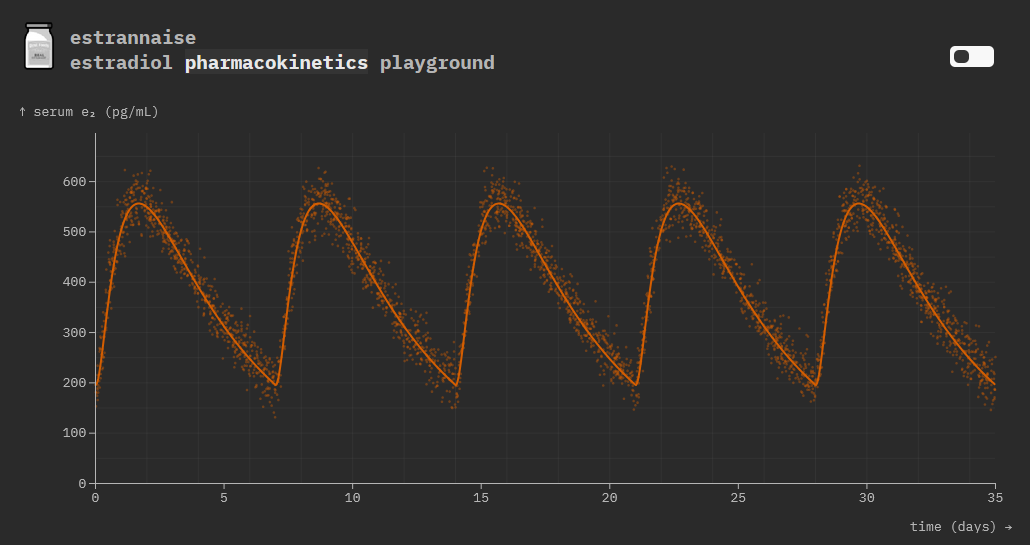
\includegraphics[width=1\linewidth]{ev.png}
     \caption{Serum Estradiol (pg / ml) of Estradiol Valerate vs Time (days) }
     \label{fig:ev}
 \end{figure}

\subsection{How do I dose \textit{estradiol cypionate}?}

\textit{Estradiol cypionate} can accommodate a weekly dosage without issue. \textbf{A weekly dosage between 5-7mg is typical.} Extending the duration past weekly (e.g., every 10 days) is not recommended because it is a less efficient use of estrogen compared to weekly as it requires increasingly higher dosages to reach acceptable levels. Any extension past weekly is much more prone to side effects due to variance (See Question \ref{7-3}).

\subsection{How is the hormone curve for \textit{estradiol cypionate} characterized?}

\textit{Estradiol cypionate} is more forgiving than \textit{estradiol valerate}. The curve does not progress as quickly with a much lower variation between high and low, but there is still a noticeable rise and fall over a typical weekly duration.

 \begin{figure}[H]
     \centering
     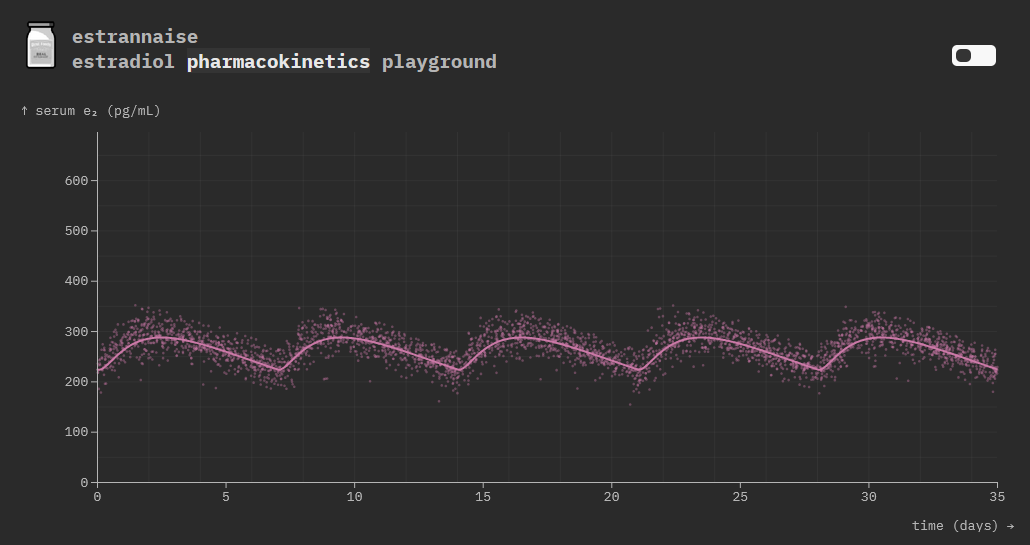
\includegraphics[width=1\linewidth]{ec.png}
     \caption{Serum Estradiol (pg / ml) of Estradiol Cypionate vs Time (days) }
     \label{fig:ec}
 \end{figure}

\subsection{How do I dose \textit{estradiol enanthate}?}

\textit{Estradiol enanthate} can easily accommodate a weekly dosage without issue and can possibly be extended up to 10 days if one is inclined. Beyond that is technically possible but not recommended as levels will become increasingly unstable. \textbf{A weekly dosage of 4-6mg is typical}, with 5-7mg recommended for up to 10 days. Weekly is still recommended regardless for consistency and ease of scheduling as any extension up to 10 days does not offer much benefit in my opinion.

\subsection{How is the hormone curve for \textit{estradiol enanthate} characterized?}

\textit{Estradiol enanthate} is the gold standard for injectable estrogen. It has a curve that is extremely flat (i.e., has little variance) over the duration of a typical weekly duration. This allows for very consistent levels without any negative side effects related to variance (See Question \ref{7-3}).

 \begin{figure}[H]
     \centering
     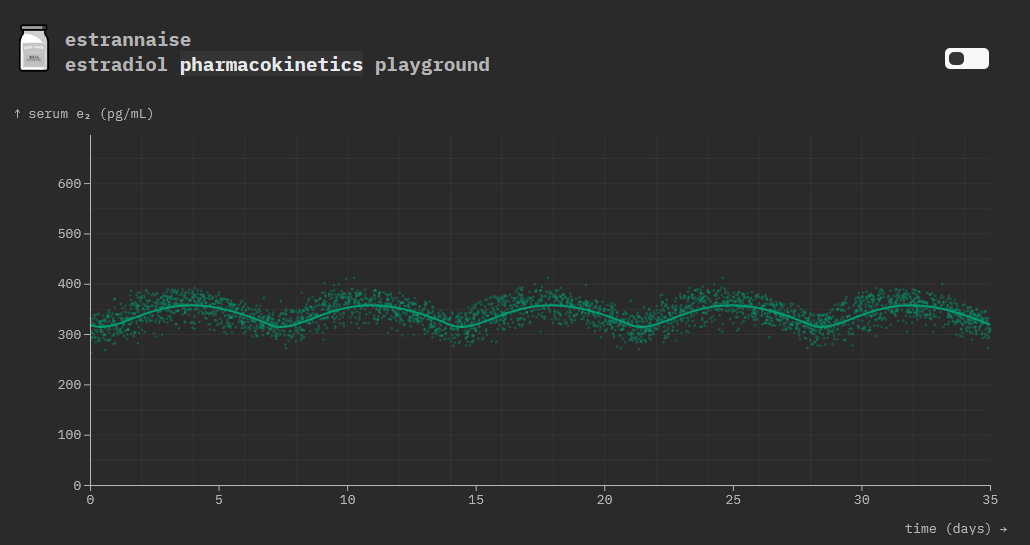
\includegraphics[width=1\linewidth]{een.png}
     \caption{Serum Estradiol (pg / ml) of Estradiol Enanthate vs Time (days) }
     \label{fig:een}
 \end{figure}

\subsection{How do I dose\textit{ estradiol undecylate}?}

\textit{Estradiol undecylate} is capable of extending far beyond weekly into the range of monthly or quarterly. The recommended dosing for this, however, is not standardized or known. The factors that affect how the estrogen from an injection is absorbed (\textit{“pharmacokinetics”}) that are negligible for other esters are significant for \textit{estradiol undecylate}. As a result, this is still highly experimental territory that is beyond the scope of this guide. Consider consulting a witch’s almanac for the lunar calendar to inject once every full moon.

\subsection{How is the hormone curve for \textit{estradiol undecylate} characterized?}

We don’t really know. The data is too sparse to paint an accurate picture of it in full, and the variables are plentiful. It is something that you can research and experiment with if you are interested, but it is new ground and you need to understand the risks involved with being a human guinea pig, so I don’t recommend it unless you know what you are doing.

 \begin{figure}[H]
     \centering
     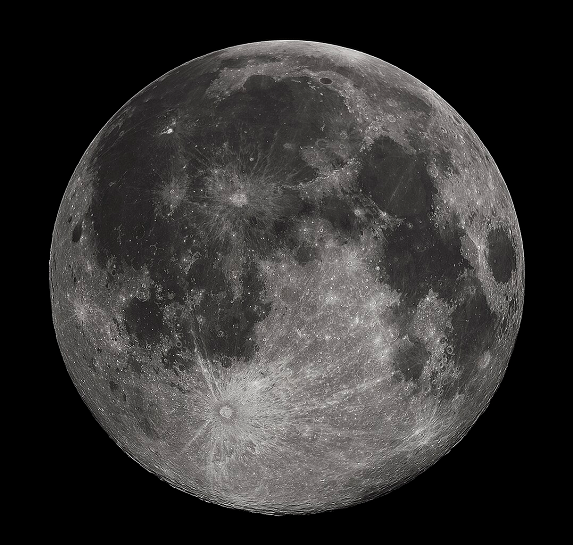
\includegraphics[width=1\linewidth]{moon.png}
     \caption{The Moon}
     \label{fig:moon}
 \end{figure}

 

\section{BLOOD TESTS AND LEVELS}

\subsection*{Acquiring Results}
\addcontentsline{toc}{subsection}{\textemdash{} Acquiring Results}

\subsection{How often should I test my levels?}

While you are first dialing in your dosage, you will want to test relatively frequently. Following any adjustment to your regimen, you should give your levels 1-2 months to stabilize, and then test once they've reached their new normal.

\subsection{Do I have to test my levels before starting HRT?}

Arguably no, because testosterone will be too high and estrogen will be too low so it’s not particularly useful data, but routine general blood tests (i.e., a lipid panel and such) are recommended for your health nonetheless. The exception is if you believe that you may have an intersex condition which may affect your HRT regimen as sometimes this can be visible in the preliminary blood test.

\subsection{Do I have to test my levels if I haven’t changed my dosage in a long time?}

Arguably no, because if you have not changed anything then nothing should have changed. It can be good for peace of mind if you have changed aspects of your routine / supplier, and doctors/insurance often require it, but major deviation shouldn’t be expected. A caveat is that if you are experimenting with \textit{estradiol undecylate}, you almost certainly should test quarterly at minimum regardless.

\subsection{I don’t have insurance or a doctor. Where can I get a blood test?}

Look into private blood testing options in your region depending on the legality of it. In many locations, you are legally able to get private blood tests, but they might not be cheap. There may be online options that allow you to get those tests at a discount but it depends heavily on your region.

\subsection{I can’t get / afford a blood test. Can I still do HRT?}

While having the information is obviously preferable to not, HRT is extremely safe and at typical dosages should pose no issue. You will just have to rely more on how you are feeling and what you observe.

\subsection{What should I test for?}

\textit{Estradiol} (E2) and \textit{total testosterone} (T) at the least because these are the main things to be concerned about. \textit{Sex hormone binding globulin} (SHBG), \textit{dihydrotestosterone} (DHT), \textit{estrone} (E1), and \textit{prolactin }(PRL) can also be useful to test if you are experiencing issues because these can be useful for troubleshooting. \textit{Follicle-stimulating hormone} (FSH) and \textit{luteinizing hormone} (LH) can tell you if your HPG axis is inactive which is the basis of monotherapy (See Question \ref{2-3}). But again: \textbf{\textit{Estradiol} and \textit{Total Testosterone} are the primary concerns. }

\subsection{When should I take a blood test during my hormone cycle?}

At the end of your cycle (\textit{“trough”}). You want as close to the bottom as possible because this is the most useful piece of information. Arguably, it is the only useful piece of information as consistent minimum levels are the primary concern. Example: If you normally inject Thursday afternoon, get your labs in the morning or early afternoon on the following Thursday before your next injection.

\subsection{My doctor said to take mid-point / peak level blood tests, should I?}

\textbf{No.} Measuring the peak estrogen level does not provide useful information and is only a measure of what ester you are using. Charitably, it is incompetence because of dated conservative standards of care. Uncharitably, it is malice to ensure insufficient estrogen levels that will result in poor health, slow results, or otherwise negative outcomes. \textbf{I recommend measuring at trough regardless.}

\subsection*{Interpreting Results}
\addcontentsline{toc}{subsection}{\textemdash{} Interpreting Results}

\subsection{What estrogen levels do I want?}

This is probably the most controversial question with transition. The short answer is that you want enough that you feel good and that you are suppressing testosterone if you need to, but beyond that, higher levels are unnecessarily wasteful at best and may be counterproductive at worst. This is a wide range however, and with so many variables there is always personal deviation. In other words: You want enough estrogen such that you feel good, and that’s it.

\subsection{Do higher estrogen levels feminize better or faster?}

\textbf{No.} Higher estrogen levels than necessary might be preferred by someone for their subjective experience, but they do not confer feminization benefits. In fact, levels that are too high can feel bad by causing mood instability or other undesirable side effects. \textbf{Minimizing testosterone levels to a baseline is far more important for feminization than maximizing estrogen levels.}

\subsection{Okay, but what number do I want to see from my estrogen lab result?}

With the understanding that the exact number does not matter, that the number will always be slightly higher than whatever is in your body even on a trough day because of latency, and that the number will be in a cloud of possibilities based on any number of factors, \textbf{I recommend a trough of about 200 pg/ml (730 pmol/L) minimum.} This is a slightly conservative recommendation to provide ample wiggle room as suppression of the HPG axis occurs below this. Around here tends to work well for most, although some prefer higher or lower. I don’t believe this is a number that should be overly fixated upon because it is inherently variable and if you feel good that is what matters most, \textbf{but} \textbf{beyond 300pg/ml (1100 pmol/L) at trough is almost certainly higher than it needs to be or should be.} There are exceptions to this, but you probably aren't the exception. Still, do what feels right. Additionally see Question \ref{11-1}.

\subsection{What testosterone levels do I want?}

Testosterone suppression is the key requirement for adequate feminization, so under 50 ng/dL (1.7 nmol/L) is generally sufficient. \textbf{Notably, near-zero testosterone is not desired.} See Section \ref{T} “TESTOSTERONE”.

\subsection{I naturally have high/low T. Do I need to adjust my dosage?}

Probably not. The testosterone range that is typically found prior to HRT is almost always higher than what is desired for feminization and will still be suppressed regardless (See Question \ref{2-3}). The exception would be if you have any variety of intersex conditions that may cause need for finer adjustment than the recommendations listed in this guide which is beyond the scope of what this guide can provide to you. You might not need to tweak, but maybe you feel better if you do. Ultimately, do what feels right. See Question \ref{9-2}.

\subsection{I have had bottom surgery. Do my estrogen levels need to be different?}

Since testosterone suppression is no longer a concern for you, you likely can still feel great with lower estrogen levels than you currently have, \textbf{but you do still need estrogen.} Because you no longer produce your own hormones, it is crucial that you still maintain sufficient hormone levels for your health. Having little to no hormones will lead to menopause symptoms which is the same reason that older cis women might take HRT once they hit menopause. Adjust as you see fit.

For additional clarity: \textbf{maintaining a minimum of about 100 pg/ml (350 pmol/L) is essential to avoid bone mineral density concerns.} If the bulk of your feminization is already complete, then in many respects your hormonal profile is comparable to a menopausal cis woman so lessons can be learned from them (See Question \ref{11-29}). In some cases of fatigue or low energy, supplementing low dosages of testosterone may be beneficial (See Question \ref{9-2}).

\subsection{Is there anything that can cause a blood test to be inaccurate?}

Depending on how the blood is measured (\textit{“assay”}), biotin supplements can cause \textit{estradiol} (E2) levels (among others, but \textit{estradiol }is our concern) to be unexpectedly high. It is not always possible to know the type of assay that will be used, so pausing any biotin supplements a few days before testing is recommended. It is also possible that there was an error with the equipment or the sample, although this is not likely.

\subsection{Do different estrogen esters or administration routes show up differently on blood tests?}\label{4-16}

No. There is no way to tell what type of estrogen someone is taking based solely on a blood test result. The various injectable esters all convert to \textit{estradiol }like we want, and the same is true for pills, patches, gels, sprays, or whatever else. It's all estrogen at the end of the day.

 

\section{TECHNIQUE AND SUPPLIES}\label{ts}

\subsection*{Sites \& Safety}
\addcontentsline{toc}{subsection}{\textemdash{} Sites \& Safety}

\subsection{How do I safely perform an injection?}

I recommend the following two videos:

\begin{enumerate}
  \item \href{https://www.youtube.com/watch?v=cBabaGC2Dok}{\textit{“How to perform an intramuscular (IM) self-injection”}}
  \item \href{https://www.youtube.com/watch?v=YfNlAZLxLyw}{\textit{“Painless (for me so far) IM Injection Technique”}}
\end{enumerate}

Between these two videos, you should be fully equipped to properly inject with minimal pain. I suggest studying them and revisiting as needed. \textbf{One key thing to emphasize is to inject with the bevel facing up to reduce pain.} In other words: the needle has a clearly defined point, and you want that to be what touches your skin first. You want a nice straight line of travel. You can think about how your hand/wrist rotates if that helps you visualize the motion, but realistically it'll be intuitive muscle memory that you'll learn naturally.

\textbf{Remember: injecting is a skill!} You will get better with time, and it won’t take long. You got this.

\subsection{Do I have to inject exactly like this?}

No, variation is fine. Ultimately when the task is just poking yourself, there’s a lot of ways to do that. Find the way that works best for you. Doing a quick dart motion usually works best, but if you have to go slow that works fine too if it’s something that is consistent that you can get better at doing.

\subsection{How do I get past injection anxiety?}

I suggest making a ritual out of the process. By forming a routine, the process becomes second nature. If you can distract your mind by listening to music, having a conversation, watching a show, or doing something else that works for you to let your muscle memory take over, that’s great! Find what works for you. Having a friend or loved one do your first few injections can help too. For most people, the first injection is the scariest. Usually people say, “Oh, that was it?” because it’s never as bad as they expect.

\subsection{Does it matter where I inject in my body?}

Yes and no. Staying within safe areas matters, but otherwise, where you inject primarily depends on your mobility, the volume of fluid that you are injecting, the needle/syringe combo that you are using, and your own comfort. Either way, \textbf{make sure to rotate injection sites.} Alternate sides of your body with every injection–for example, if you inject into your right leg one week, use your left leg the next. This is to minimize any long term scarring risks.

\subsection{What injection sites are safe?}

Opinions vary between medical authorities, but your body composition can also play a role. I recommend injecting on the side of the leg as shown in the video(s) because it is doable for most people and is capable of being very consistent which means consistently painless injections once your technique is practiced, but other people prefer their glute or their stomach. \href{https://vertisis.com/articles/how-to-self-administer-a-subcutaneous-injection}{This video and website} shows other injections sites that can be acceptable depending on the supplies you use. Figure out what works best for you.

\subsection{What do “intramuscular” (IM) and “subcutaneous” (SubQ/SC) mean?}

You will often hear these terms in the context of injections. \textit{Intramuscular} means injected into the muscle and \textit{subcutaneous} means injected into the fatty layer beneath your skin.

\subsection{What is the difference between intramuscular injections (IM) and subcutaneous injections (SubQ/SC)?}

\textbf{In the context of HRT, there is little to no difference between intramuscular and subcutaneous injections.} Subcutaneous injections are absorbed more slowly than intramuscular injections, however this is generally not significant enough of a difference to impact dosing. It should also be noted that an injection is rarely deposited fully in muscle or fully in the subcutaneous layer which blurs any difference together even further on an injection-by-injection basis.

As a side note, pharmaceutical sources for estradiol vials typically say they are for intramuscular injections only because that is what they are technically approved for. It does not matter though.

\subsection{Should I perform intramuscular injections (IM) or subcutaneous injections (SubQ/SC)?}

\textbf{This is the wrong question.} \textbf{An injection is an injection.} Subcutaneous injections are often recommended because people believe that they allow for less painful injections by virtue of being subcutaneous, but there is not a fundamental difference in how an injection is performed. \textbf{The advantages that people refer to are not inherent to the injection depot location; they are inherent to the factors that affect injection pain.} The better question would be “How do I minimize pain during injection?”, but two other questions first.

\subsection{Does my injection angle and/or preferred injection method matter?}

No. To reiterate, the most important part of performing an injection is that you pierce a needle through your skin and deposit fluid into your body. If the fluid doesn’t leak out (or at least, not much) and it doesn’t hurt (or at least, not much), then you have done a fantastic job. \textbf{I cannot stress enough that the intramuscular vs subcutaneous “divide” is nonexistent and that the question does not meaningfully impact the effectiveness of injectable estrogen.} \textit{Estradiol undecylate} is the only case where depot location seems to meaningfully affect absorption, but even then, we don’t fully understand the details. Point being: please be concerned about the things that matter and not the things that don’t matter.

\subsection{Do I have to aspirate?}

No. “Aspiration” refers to pulling the plunger back after puncturing the skin before injecting the fluid with the intent of ensuring a blood vessel is not being injected into. Its necessity is controversial, but for hormone injections following standard procedures, there are few benefits that outweigh the negatives. The standard injection sites have low risk of striking a blood vessel in the first place, lessened even further by shorter needle lengths, so this practice is not recommended anymore by most medical organizations.

\subsection{How do I minimize pain during injection?}

Aside from practicing your technique and improving your skill, the main factor for injection discomfort is the needle and syringe combination that you are using. \textbf{To minimize discomfort, the highest needle gauge that your vial’s carrier oil is capable of tolerating should be used along with an appropriately sized syringe and needle length. }You should ask “What needle gauge and length should I inject with?” To answer that, let’s talk about how needles work.

\subsection*{Knowing Your Needles}
\addcontentsline{toc}{subsection}{\textemdash{} Knowing Your Needles}

\subsection{What is “needle gauge”?}

\textit{Needle gauge }is a measure of needle thickness. The bigger the number, the thinner the needle. A 25G needle is thinner than a 20G needle, for instance. Higher gauge needles also tend to be shorter because longer needles become more prone to bending, so their length has a lower maximum. Unsurprisingly, thinner needles generally hurt less. It should be noted that the gauge of needle(s) used will not affect HRT in any way; it will only affect the ease and comfort of the injection itself.

\subsection{What are “Luer lock” and “insulin” syringe/needles?}\label{5-13}

\textit{Luer lock syringes} have separate syringes and needles so a separate needle can be used for drawing and injecting. \textit{Insulin syringes} have a needle fixed in place which means that the same needle will be used for drawing and injecting. Note: You do not want “Luer slip” needles as they are prone to error. Where possible, insulin syringes are preferred for comfort and for minimizing dead space (See Question \ref{5-26}).

\textbf{Safety Warning: Recapping needles is generally not recommended out of concern for sticking yourself, but if you do (such as when swapping out a drawing needle), NEVER apply force with your hand towards the needle.}

It is possible that the cap may break and you may injure yourself if you place the cap incorrectly. Gently “scooping” the cap onto the needle off of a horizontal surface and pressing the loosely capped needle against a wall or pulling the cap on the sides to fully seat the cap is preferred. There isn't a disease transfer risk when performing a self injection, so heed this warning at your own discretion, but resticking is a VERY serious concern when performing injections on others. For disposal, see Question \ref{5-27}.

\subsection{What needle gauge should I draw with?}

If you are using Luer lock syringes, it is recommended to use a lower gauge than what you inject with so that it takes less time to draw from the vial. Too low can lead to coring (See Question \ref{5-23}), so at least 21-23G is recommended. If you have patience and lower volumes to inject, then higher gauges are recommended for the aforementioned coring risk reduction. Please note that the needle does not meaningfully blunt on the stopper. This question is irrelevant with insulin syringes because the needle is not removable.

\subsection{What needle length should I draw with?}

If you are using Luer lock syringes, the length of the drawing needle does not matter too much outside of the inconvenience of having too long of a needle being unwieldy. In other words, no need to be picky. This question is irrelevant with insulin syringes because the needle is not removable.

\subsection{What needle gauge should I inject with?}\label{5-16}

This is a tricky and highly subjective question, and your answer will depend on 4 main factors: 1) the carrier oil for what you are injecting; 2) if the vial contains a cosolvent; 3) your patience to have a needle in your leg for longer; and 4) your willingness/ability to push harder on the syringe plunger. It’s a question of comfort. Thicker oils mean more time and more effort when using a higher gauge, but also higher gauges can be significantly less painful going in. \textbf{As a baseline, 25G is the minimum needle gauge that you should use to manage discomfort. }Most common carrier oils can generally do up to 27G comfortably, whereas MCT oil in particular is notable for being able to easily do 30G (See Question \ref{6-16}).

\subsection{What needle length should I inject with?}

\textbf{I recommend between 0.5” to 1” (12.5mm to 25mm) depending on your gauge.} Below 0.5” (12.5mm) increases the likelihood of leakage. 0.25” (6.5mm) length needles can be fine depending on your technique and the fluid you’re injecting, but 0.5” (12.5mm) is a safe bet. Beyond 1” (25mm) is unnecessarily daunting and painful without any added benefits.

\subsection{Does syringe size matter?}

\textbf{Yes, size matters.} There are two reasons for this. 1) Higher volume syringes tend to be less precise which leads to incorrect dosing, and 2) physics makes higher volume syringes more difficult to inject. For dosing accuracy, you do not want to use a syringe far larger than the volume that you are injecting (i.e., for injections less than 0.1ml, get smaller than 1ml syringes). \textbf{Avoid 3mL syringes entirely if you can.} Obviously use them if it’s all you have, but they’re really not meant for a task like this. Do not ask me why pharmacists seem to near-exclusively hand them out. A cruel joke, maybe.

\subsection{Where do I buy syringes and needles?}

It depends on your local jurisdiction as some localities ban the sale of needles and syringes to individuals as a punitive measure against drug users. Otherwise, medical and veterinary supply businesses or authorized manufacturer retailers should be good places to look. \textbf{Amazon is not recommended} because the quality is uncertain.

\subsection{Is it okay if I reuse needles or syringes?}

\textbf{No. Never reuse needles or syringes. }Or share either. You probably already know this but I’m just reminding you because it’s really not good or safe to do!

\subsection{What if I want to do injections but have difficulty performing it on myself?}\label{5-21}

You might like an auto-injector. As the name suggests, auto-injectors perform the injection for you. Auto-injectors like the \href{https://unionmedico.com/90-super-grip/}{\textit{UnionMedico 45/90 Super Grip}} can take 1ml syringes which can take the difficulty out of injecting (but you still manually press the plunger), whereas auto-injectors like the \href{https://www.owenmumford.com/us/medical-devices/autoject-2}{\textit{Owen Mumford Autoject 2}} entirely hide the needle of an insulin syringe and automatically push down the plunger. There are also a variety of 3D printable designs available online. I have used none of these products and these are not endorsements.

\subsection*{Basics of a Vial}
\addcontentsline{toc}{subsection}{\textemdash{} Basics of a Vial}

\subsection{What should I look for when inspecting vials?}

Aside from looking for signs of coring (see below), you should look for any signs of discoloration, separation, contamination, crystallization, cracks in the glass, fibers, hairs, etc. A properly made vial should not deviate too much from usual. \textbf{Always inspect your vials before use. Do not use a vial that does not seem right.}

\subsection{What is “coring”?}\label{5-23}

\textit{Coring} is when a piece of the rubber stopper breaks away and falls into the vial. This can occur with too large of drawing gauges, repeated punctures on the exactly same spot, or too many punctures (i.e., a very small volume injection with a very large volume vial). \textbf{A cored vial should be immediately discarded. }The \href{https://www.youtube.com/watch?v=w5F0SLoMjC8}{\textit{45-90° technique}} can also be used to help minimize coring.

The concern with coring is that you do not want to inject bits of rubber into you. If there are large bits of rubber, there might be smaller ones that you can't see. The purpose of the stopper is to protect the contents from the elements, so a vial with a hole in the top is more prone to oxidation and/or bacterial growth. \textbf{As a side note: Please ensure that you remove the metal or plastic cap off the top of a new vial. }This may seem obvious, but some vial designs can be confusing. 

\subsection{How long until a vial expires?}

A sealed vial could last for years without issue if it is stored at stable temperatures away from the light. Concerns with age are primarily carrier oil oxidation assuming that the vial was sterilized as it should be. A punctured vial that has a preservative in it (See Question \ref{6-17}) should last at least a year or whatever the life time of the vial is (i.e., how long until you use it all). The “discard after 28 days” listing on vials is simply the minimum requirement for how long manufacturers must guarantee sterility, not the maximum shelf life. 

\subsection{How should I store a vial?}

Stable room temperature and away from light. High heat and UV can cause degradation of the carrier oil, whereas low temperatures can cause crystallization. Crystals can be dissolved and reincorporated, but it’s a potential cause for irritation if they aren’t fully dissolved. This goes for both sealed and unsealed vials.

\subsection{What is “dead space”?}\label{5-26}

\textit{Dead space} refers to the amount of fluid that is wasted when performing an injection. This is fluid that is trapped in the syringe or in the needle. With a standard Luer lock needle/syringe this can be up to 0.1mL, whereas in an insulin needle can be as low as 0.003mL. Reducing dead space is recommended for economic reasons because it adds up to a lot of wasted estrogen. \href{https://hrtcafe.net/Calc/}{This calculator} can be useful for estimating how much estrogen is wasted depending on the supplies used.

One thing to note if you are swapping needles for drawing and injecting, then you should pull the plunger back slightly prior to taking off the drawing needle so that the fluid inside the drawing needle is not wasted. It is very minor, but it can make a difference. See Question \ref{7-7} for another possible strategy if concerned about high dead space.

\subsection{What do I do with my used syringes and needles?}\label{5-27}

Place all used injection supplies pointed down in a sharps container (either a dedicated biohazard container or reusing hard plastic tubs such as from protein powder or laundry detergent). When the container becomes three-quarters full, seal it closed so that it cannot be accidentally opened. Clearly label it “USED SHARPS” and then dispose of it according to your local jurisdiction's requirements. \textbf{Note that sharps should NOT be placed into trash or recycling containers.} Your city/state/region likely has a website somewhere describing how and where to dispose of household hazardous waste. For the US, \href{https://safeneedledisposal.org/}{you can go here.}



\section{SOURCING VIALS}\label{sv}

\subsection{Where do I get estrogen vials to inject?}

Broadly speaking, you have two options: \textit{pharmaceutical sources} and \textit{DIY sources}. \textit{Pharmaceutical sources} typically require a doctor's prescription because HRT is not available over-the-counter (or if it is, vials are not included) in most countries. \textit{DIY sources} encompass everything else.

\subsection{Should I use pharmaceutical sources or DIY sources?}

The choice is yours, but sometimes there is no choice at all. There are pros and cons to each. Of course, there is nothing stopping you from procuring estrogen from multiple sources to get the benefits of both. In many situations, it may be recommended.

\subsection*{Pharmaceutical Sourcing}
\addcontentsline{toc}{subsection}{\textemdash{} Pharmaceutical Sourcing}

\subsection{What are the pros of pharmaceutical sources?}

\begin{itemize}
  \item Can generally trust quality control processes and certifications;
  \item Insurance may cover it in part or in full;
  \item Can be more convenient depending on your luck with doctors;
  \item The product most likely will be consistent;
  \item \textbf{At least appearing to be using pharmaceutical sources may be required if you are seeking insurance approval for surgeries.}
\end{itemize}

\subsection{What are the cons of pharmaceutical sources?}

\begin{itemize}
  \item Reduced (or no) selection of esters;
  \item Possible lengthy wait time (months or years);
  \item May be required to have a prescription (depending on country);
  \item Insurance may not cover costs in part or in full;
  \item May not be prescribed at all in your country;
  \item Your doctor may arbitrarily refuse to prescribe it to you;
  \item Your doctor may arbitrarily withhold refilling a prescription;
  \item Shortages may prevent filling a prescription at all;
  \item Likely held to stringent WPATH requirements or worse;
  \item Harder to stockpile;
  \item Access is subject to the whims of your country’s political situation which also means that your transness will likely be included on your medical record. 
\end{itemize}

\subsection*{DIY Sourcing}
\addcontentsline{toc}{subsection}{\textemdash{} DIY Sourcing}

\subsection{What are the pros of DIY sources?}

\begin{itemize}
\item Generally much cheaper in most places;
\item Available anywhere in the world;
\item Obtaining it can take months or even years less time than waitlists (the only wait is shipping and production);
\item Easy to stockpile;
\item Full selection of esters;
\item No requirement of dealing with the medical system;
\item It’s probably made with love.
\end{itemize}

\subsection{What are the cons of DIY sources?}

\begin{itemize}
  \item Almost certainly not made in a certified clean room;
  \item Quality can vary depending on the source;
  \item Can be inconvenient depending on the source;
  \item Requires trusting the source;
  \item Requires finding a source;
  \item Sources are more likely to close than your local pharmacy;
  \item Product delivery times can vary;
  \item Most likely have to use cryptocurrency which is annoying;
  \item Cannot use insurance if that was an option for you.
\end{itemize}
Additionally as already stated, if you are seeking insurance approval for surgeries, they likely require a minimum amount of time with an HRT prescription. This may or may not be a concern for you.

\subsection{What types of injectable estrogen are DIY only?}

Chiefly, \textit{estradiol enanthate}. Pharmaceutical sources will almost always prescribe you \textit{estradiol valerate}, but not always at a 40 mg/ml concentration. \textit{Estradiol cypionate} may occasionally be prescribed, but rarely above 5 mg/ml or 10 mg/ml concentrations, which are annoying to dose. The benefits provided by \textit{estradiol enanthate} alone are very good reasons to consider DIY, but you can get any ester at 40 mg/ml from DIY sources.

\subsection{What actually \textit{are} DIY sources?}

DIY sources include commercial brewers, mutual aid projects, your friend, and yourself if you have an entrepreneurial spirit!

\subsection{Where can I get DIY vials?}

What are you, a cop? I’m not telling you that. That’s not the point of this guide anyways. There are other resources that have that information. Stay focused.

\subsection{How can DIY sources be cheaper than pharmaceutical sources?}

The cost to produce a vial is roughly around \$10, including labor and amortized capex cost. This is likely a high estimate. The bulk of the cost for commercial DIY sources are the layers of overhead and shipping involved in anonymity. Non-commercial DIY sources likely have no such overhead. Pharmaceutical sources generally do not have any incentive to be cheaper than what they are. 

\subsection{Is DIY legal?}\label{6-11}

In most locations including America, estrogen is not a scheduled substance, whereas testosterone may or may not be criminalized. The US is an anomaly for testosterone in this regard, as other countries don’t criminalize possession of testosterone, but prosecution is rare anyway given the wide availability of steroids. \textbf{This guide is not legal advice.}

\subsection{Is DIY safe?}

“DIY” as a broad category of sources is neither safe nor unsafe, but not all DIY sources are equal. When we are discussing the topic of safely injecting something into your body, the real question is: do you trust that the person who produced that vial properly followed aseptic techniques and procedures such that the vial contains what you want and nothing else? For pharmaceutical sources, that trust is innate on the assumption that laws and regulations exist. For DIY sources, that trust must be earned through demonstration/explanation of process, independent third-party testing for concentration/purity, and community reputation.

\subsection{What things should I look for to know if a DIY source is trustworthy?}

Use your gut and your brain. 

\begin{itemize}
  \item Are they open to talking to you about their process / have it listed somewhere? (e.g., do they filter for dust? The answer should be yes!!!)
  \item Do they seem competent in their ability?
  \item Have they had their product tested? 
  \item Are they a trusted member of the community?
  \item Have they been vetted or vouched for by other members of the community who you trust? (i.e., inspections, reviews, testimonials, etc)
  \item Mistakes happen, but do they take accountability or do they try to silence negativity?
  \item For commercials, do they resolve any issues with customer orders?
  \item For commercials, are they taking payment on product not yet produced without indicating that it is a backorder? (You should never backorder!)
  \item Do their vials contain preservatives?
  \item How long have they been producing? (For good reason, they may not tell you!)
  \item How much do they produce? (For good reason, they may not tell you!)
  \item Are the vibes just \textit{off}?
\end{itemize}

These are just some of the many questions that can be asked to know if you trust that they care as much as you do about the quality of their product.

\subsection{Should I hold different DIY sources to different standards?}

Likely, yes. Commercial brewers should also be held to a high standard if you are giving them money in exchange for product because they can afford to do it right. A mutual aid product on the other hand that is distributing vials for free might not be something that you can afford to be picky about, although that is not to say that the product is likely to be better or worse. As for a friend or yourself, only you can decide that!

\subsection*{Anatomy of a Vial}
\addcontentsline{toc}{subsection}{\textemdash{} Anatomy of a Vial}

\subsection{What should I look for in a vial?}

The ingredients inside of a vial can be categorized as \textit{“active”} and \textit{“excipient”}. The\textit{ active} is the estrogen ester in our case, and the \textit{excipients} are everything else. There are generally three or four ingredients: 1) the estrogen ester; 2) the carrier oil; 3) the preservative; and optionally, 4) any cosolvent(s). We have already covered the estrogen esters in Section \ref{td} “TYPES AND DOSAGES”. Pharmaceutical vials almost always have all four ingredients.

\subsection{What carrier oil should I look for in a vial?}\label{6-16}

This is a question of preference, personal tolerance, and possibly allergies. \textbf{The main variable relevant to you is viscosity because that affects injection comfort and convenience.} As discussed (See Question \ref{5-16}), thinner oils are able to more conveniently use higher gauge needles without difficulty when drawing and injecting. \textbf{The most commonly used carrier oils for HRT are castor oil and MCT oil. }Castor oil is the thickest oils commonly used, but it also tends to result in the least amount of irritation so pharmaceutical vials typically use it. MCT oil is the thinnest oil commonly used, but some people find it more irritating than other oils and it’s DIY only. Cottonseed oil and grapeseed oil occasionally find use, but usually not by HRT manufacturers. Other oils like sunflower or sesame or whatever else occasionally find use but aren’t generally recommended. Depending on your circumstances, this question might not matter to you, you might not have a choice, or it may be a strict requirement. 

\subsection{What preservatives should I look for in a vial?}\label{6-17}

The most common preservative used in injectable vials is \textit{benzyl alcohol} (BA) in low concentration. This is mandatory and not up to debate. \textbf{You should never use a vial without a preservative. }For people with the rare allergy, \textit{chlorobutanol }is an alternate commonly used preservative, but almost never by DIY sources which would necessitate hunting specific pharmaceutical formulas.

\subsection{What cosolvents should I look for in a vial?}

The main cosolvent used is \textit{benzyl benzoate} (BB) which reduces the viscosity of the resulting solution. This is technically optional, but it is generally recommended for batch consistency and in many cases is necessary depending on the carrier oil and the desired concentration. Some people find it irritating, but others don’t. 

 

\section{TROUBLESHOOTING}

\subsection*{Dosage Uncertainty}
\addcontentsline{toc}{subsection}{\textemdash{} Dosage Uncertainty}

\subsection{My levels aren’t what I expected them to be. Why not?}

There are a number of possibilities. Recall first that model estimations cannot take into account any plethora of factors which may cause some deviation. Recall as well that it takes multiple injections until you reach stability, so if you just changed your dosage that may be why. Quadruple check with a friend that you are injecting as much as you think you are. That is more commonly an issue than you might think, but for DIY sources it is also possible that the concentration is lower than advertised due to inexperience or less precise equipment. In that case, injecting you may just need to inject a little more for that vial. \textbf{But remember, the most important thing is how you feel, not your levels. }Please note that even professional compounding pharmacies can produce dud vials not caught by quality control, as hopefully rare as that may be!

\subsection{Can I compare levels across different tests if I didn’t test at trough?}

\textbf{No.} Not accurately, anyway. This is part of why you should always test at trough. Hours before your normal time for your next injection; that’s what you want. Eliminating as many variables as possible makes the data far more useful to you. If there is nothing else that you take from this guide, please just test at trough.

\subsection{I feel really bad on my trough days. What should I do?}\label{7-3}

In most cases, either the dosage is too low or the frequency is too low. This is most pressing for \textit{estradiol valerate} and \textit{estradiol cypionate}. Adjust your dosage within the range listed or adjust the frequency. Find what works for you. It is also possible with \textit{estradiol valerate} in particular that your dosage might actually be too *high* instead of too low as the high level variability across your cycle may be the culprit for this crashing sensation. In short: swap to \textit{estradiol enanthate} if you can.

\subsection*{Injection Woes}
\addcontentsline{toc}{subsection}{\textemdash{} Injection Woes}

\subsection{The injection is harder to do when it’s cold. What should I do?}

Warm up the vial before drawing, then warm the syringe before injecting. Rolling the barrel of the syringe between your hands should be plenty to warm up the fluid. Forming this as a habit all the time should improve your injection consistency.

\subsection{The injection hurts more when it’s cold. What should I do?}

Warm up your leg before injecting. Relaxing the muscles with a massage or a hot shower (specifically: increasing the temperature with the water aimed at your leg before you get out) before injecting can help.

\subsection{I bled after my injection. Will I die?}

No. This means that you likely just hit a vein or a capillary which can happen sometimes. You might experience some light bruising or increased soreness. Using a cute bandage will make it heal faster.

\subsection{There was some air in my syringe. Will I die?}\label{7-7}

No. While you obviously do not want to inject just air and it can affect dosage if there is too much in the syringe, a small amount of air under 0.1ml is almost certainly not going to cause issue for you. It might actually be recommended in some cases. For instance, the \textit{air lock technique} (a standard technique for injecting fluids that are irritating or can stain, not crucial knowledge for HRT) generally involves injecting 0.1-0.3ml of air, so you have nothing to be worried about. You aren’t doing intravenous injections.

\subsection{Some of the fluid leaked out. Was my injection wasted and/or will I die?}

No. Leakage can happen for any number of reasons and is rarely enough to make a difference, so you do not need to do another injection. For the future, make sure to leave the needle in for 5-10 seconds before retracting and then apply pressure afterwards. You might consider using the air lock technique mentioned above if you are particularly concerned about leakage.

\subsection{Sometimes I am really sore after an injection. Will I die?}

No. Assuming you have otherwise followed all of the suggestions within this guide, sometimes the deposit of fluid hits an uncomfortable place for one reason or another. Better luck next time. \textbf{Make sure you alternate injection spots!} You do not want scar tissue to build up over the long term, and if a spot is already sore, you do not want to make it more sore.

\subsection{I am experiencing a lot of itchiness and irritation after injecting. Will I die?}

Probably not. There are a number of possible causes. Infection is the most concerning cause, but is unlikely in most cases. \textbf{Immediately go to a doctor if you are experiencing a fever, severe pain, muscle aches, pus, red streaks, or other signs of infection. }In most cases however, irritation like itchiness, redness, light swelling, warmth, etc are the result of using a vial whose estrogen and oil have separated (“crashed out of solution”). See below. It’s possible that you may be having a reaction to the carrier oil, but if you are suddenly experiencing issues after some injections without any issue, it is most likely that the vial contents are out of solution.

\subsection{My vial has crystals in it. Can I still use it?}

It most likely means your vial got too cold. Warm it up and gently shake to reincorporate. If the crystals are not going away, then it’s possible the vial contents have separated entirely. With a lot more heat and stirring the crystals might reincorporate, but it is simplest and safest to replace the vial if you can.

 

\section{PROGESTERONE}

\subsection{Do I want to take progesterone?}

\textbf{Probably.} This is a controversial question for some reason. Detractors (namely, doctors) will argue that there’s no studies to show that it plays a role in feminization therefore it should not be taken. Aside from transfeminine subjects being woefully understudied, heuristically speaking, progesterone is a key female sex hormone that plays an important role in the brain and in many functions throughout the body. Regardless of physical feminization, it is an important hormone for good health that should not be lightly overlooked.

\subsection{What is the difference between “progesterone” vs “progestin” / ”progestogen”?}

The class of hormones, both natural and synthetic, that activate the progesterone receptor are “proges\textbf{togens}”. The natural, bioidentical, and most important progestogen is “proges\textbf{terone}”. Synthetic progestogens are “proges\textbf{tins}”. These three terms are mistakenly used interchangeably in scientific literature and in clinical settings, likely causing much of the broader confusion regarding the role of progesterone in HRT, despite the fact that they are \textbf{not }equivalent.

\subsection{Do I want progesterone or a progestin?}

Progesterone. You want bioidentical progesterone.

\subsection{What’s wrong with progestins?}

Progestins, most typically \textit{medroxyprogesterone}, \textit{medroxyprogesterone acetate}, or \textit{levonorgestrel}, are generally associated with the negative side effects and long term risks (breast cancer, blood clots, depression, etc) that are falsely attributed to progesterone. They are not bioidentical which means they do not behave the same as progesterone and thus cannot be directly compared.

\subsection{What does progesterone do for feminization?}

Progesterone is believed to play a role in breast development and libido in particular, but as mentioned it’s a key hormone aside from its outward appearance effects. It does also have some antigonadotropic (i.e., it contributes to testosterone suppression) properties which can be sometimes relevant.

\subsection{Does it matter when I start progesterone?}

It is unknown. There is some belief that starting too early may harm breast development long term, but this is purely theoretical and contrary anecdotal evidence makes the answer unclear. The conservative estimate is waiting roughly a year into HRT (until Tanner Stage 3 or 4) in the possible chance that it does matter.

\subsection{How is progesterone normally taken?}

Aside from topical applications, the main form is via a pill. It is prescribed as an oral pill but is most effective when taken as a suppository. Topical sprays and creams can also work very well.

\subsection{Are you serious that progesterone should be taken as a suppository?}

Progesterone metabolizes entirely differently when taken orally vs rectally due to passing through the liver when taken orally. Oral progesterone primarily converts to \textit{allopregnanolone} which can cause heavy drowsiness, whereas rectal progesterone primarily converts to progesterone itself which is what we want (although some still converts). Some people take additional oral progesterone as a sleep aid, but please note that too much \textit{allopregnanolone }can sometimes lead to negative mental health side effects.

\subsection{How do I take progesterone as a suppository?}

Just a bit of water on the pill should work, then dry off and wash your hands. Obviously, don’t go to the bathroom for the next hour or so, so doing it before bed is best. If you are having issues with it not dissolving then you can try piercing the capsule but usually should be no issue. Be aware that if you use large homebrew suppositories made using coconut oil, the large volume of coconut oil will not want to stay in you.

\subsection{How much progesterone should I take?}

For pills, Standard dosage is 100-200mg daily at night. It is a rather arbitrary dosage; 200mg is the max that most doctors will prescribe. Some people take more than 200mg on occasion, but be aware that spiking your levels may lead to an unpleasant crash. See question below.

For topical applications, nobody can tell you with certainty due to the high variability of the delivery medium, nor is there any clear guidance on desired levels, or even frequency (likely daily), as progesterone is simply understudied. Because of this, I would advise titrating your dosage so that you understand how progesterone affects you.

\subsection{Is there any benefit to “cycling” progesterone?}\label{8-11}

No. Some people do this to mimic a cis woman’s menstrual cycle, but there is no reason to believe there is any benefit to this and it may cause negative PMS symptoms. The only exception is if you have good reason to suspect that you have an intersex condition involving a uterus that you are managing. I discourage it otherwise. See Question \ref{11-10}.

\subsection{How long should I take progesterone for?}

For as long as you plan to take estrogen and for as long as you want to. So, probably forever.

Sometimes people (or doctors) arbitrarily say to only take progesterone for X years. There is zero theoretical or empirical reason to suggest that this is sound advice. It's about as coherent as if someone (or a doctor) asked how long a trans person planned to take HRT for\textemdash{}oh wait never mind they do ask that.

\subsection{Can progesterone convert into \textit{dihydrotestosterone} (DHT)?}

No. Well, strictly speaking yes, but also no. It is largely a myth, although \href{https://whsah.co/posts/rethinking-progesterone-and-androgens/}{as outlined in detail by alix in this article}, for cases of people with \textit{nonclassical congenital adrenal hyperplasia} (ncCAH) progesterone can cause some negative side effects of increased androgenic activity. In those cases, discontinuing progesterone is recommended along with seeking out a formal diagnosis/treatment for potential adrenal disorders.

\subsection{Is there any benefit to topical progesterone applications in addition to pills?}

Maybe. It's a possible alternative to pills, especially in the case of someone with a peanut allergy since the most common pill manufacturer uses peanut oil, but again dosage is unclear. Some people find more progesterone fun, if nothing else. Be safe and have fun.

For clarity: Apply creams to your inner thigh region (elsewhere if directed), or optionally on scrotal skin (it's thin and highly vascular) in the case of sprays. And no, applying progesterone to your breasts directly is unlikely to make them grow bigger or faster compared to otherwise. 

\subsection{Can I snort progesterone powder?}

Please don’t. It’s hell on your sinuses. It isn’t hard to make your own topical progesterone spray and there are guides out there. Do that instead. It’s significantly more effective, consistent, and safer.

\subsection{Where can I get progesterone?}

Progesterone tends to be more expensive through DIY sources due to the higher mass of hormones required, so ideally get it through pharmaceutical sources covered by insurance. There is also the option of grey market foreign pharmacies, which are simply pharmacies in another country, although these often require some hurdles to purchase from. Topical progesterone creams are available OTC in some locations, although it is not always the most economical depending on the concentration.

\subsection{I would like to read more about progesterone in an HRT context. What resources should I read?}\label{8-17}

Originally I linked a document here but I opted to remove it due to a number of faults that can be misleading. The problem with progesterone is that literally nobody agrees about a single aspect of it. I don't know a single source or study that people agree is good. Hell, people don't even agree if the word starts with the letter “P”. \textbf{The crucial thing to know is that progesterone is not strictly required for full feminization or good breast development, but assuming that it's not contraindicated for you, it's probably worth taking.}

It should be noted that for the entire category of progestogens there are countless myths and falsehoods invented whole cloth by both proponents and detractors alike which does not make discerning truth from the already-sloppy scholarship any easier. Fantastical claims of magical benefits and fearmongering of alleged risks based on nothing are both equally unhelpful, although the later is worse in my opinion when comes from a medical authority, whether neglectful or malicious.

\subsection{Does progesterone interact with any other drugs related to HRT?}\label{8-18}

If you are taking 5$\alpha$-Reductase Inhibitors like \textit{finasteride} and \textit{dutasteride} (See Section \ref{AA} “ANTIANDROGENS”, or keep reading), these can affect how progesterone naturally breaks down into \textit{allopregnanolone} which can cause adverse mood effects in some people, irrespective of how you are taking progesterone. It is not fully clear how much the administration route for the 5$\alpha$-Reductase Inhibitors (i.e., topical vs oral) makes a difference, but lower systemic absorption via topical application may mitigate these side effects. It is recommended to not take either of those if you are someone affected by this interaction, but it is not in all cases anyway. Note that these depressive effects may be felt for up to a month after stopping. 
 

\section{TESTOSTERONE}\label{T}

\subsection{Why don’t we want zero testosterone?}

Testosterone is an essential sex hormone which plays a key role in your health and well-being. We want to suppress it for feminization, but near-zero testosterone (less than 10 ng/dl, or 0.35 nmol/L) can cause issues such as poor libido, low energy, low strength (fatigue beyond just the strength loss of HRT), poor concentration, trouble sleeping, etc. Notably, issues very similar to having too little estrogen. Cis women also have more than zero testosterone, so that need not be the fear. \textbf{Adequate hormone levels are important!}

\subsection{Are there ever cases where I would want to supplement testosterone?}\label{9-2}

Yes. If you are experiencing the issues of the above and your estrogen levels are otherwise good, it’s possible that you might want to supplement with a microdose of testosterone. If you wanted to improve your erectile function, minimize any atrophy before bottom surgery, or otherwise wanted to experiment with your hormones to see what feels best for you, then that might be a reason to explore testosterone in a different context that you can hopefully appreciate more compared to pre-HRT.

\subsection{If I wanted to supplement testosterone, how would I do it?}

There’s a few possibilities. Testosterone comes in either injections or topical gels/creams, similar to estrogen as already discussed. Topical is more likely what you are going to be prescribed. Topical applications have the downsides that we have discussed for estrogen, but those are less of a concern here when precise levels are less important.

\subsection{What are the topical forms of testosterone?}

There is gel and cream. Gel is typically what will be prescribed, but some compounding pharmacies are able to make low-penetrating cream if someone wanted just topical application on the genitals. The latter is harder to get and generally more expensive, however.

\subsection{Does it matter where I apply the testosterone?}

It depends on if you have gel or cream. If you have the kind of localized cream as mentioned above, you would apply it as directly as mentioned. Otherwise, shoulders and upper arms are where gel should go. Make sure not to touch things until long after it dries!

\subsection{How much and how often should I apply testosterone?}

Season to taste. This largely depends on how you are feeling. If you have too much, you might start to experience side effects of testosterone (e.g., oily skin and body hair), but only you can say what is preferred for you. A weekly injection of 5-10mg of \textit{testosterone cypionate} might work for you, but in the case of 1\% topical gels which are often disbursed in 25/50mg packets, there is more variability. You almost never want even half a packet, and definitely not daily. I would suggest starting with much less than you think to see how you feel.

\subsection{Where would I get testosterone?}

If you are an American, you would have to get a prescription or ask any juicer at your closest Planet Fitness. Elsewhere, it depends on what gym chain is closest to you. Disclaimer: This is a joke. See Question \ref{6-11} “Is DIY legal?”

\subsection{Are other steroids equivalent to testosterone in an HRT context?}

Anabolic-androgenic steroids, i.e., drugs that are structurally similar to testosterone, are not all equivalent. Commonly used black market steroids like \textit{trenbolone acetate} have a laundry list of undesirable side effects, but steroids like \textit{nandrolone decanoate }are occasionally used for postmenopausal cis women due to their relatively low androgenic properties which make them very favorable for transfeminine individuals. Regardless, in America it is unlikely you will be prescribed anything other than testosterone itself, if you are able to get a prescription at all.

\subsection{What is the relationship between testosterone and \textit{dihydrotestosterone} (DHT)?}

\textit{Dihydrotestosterone} is primarily synthesized from testosterone via the 5$\alpha$-Reductase enzyme with around 5\% of testosterone in your body being converted. Generally speaking, if testosterone levels are suppressed (or if you have had bottom surgery) then there should not be much left to convert, but systemic levels won’t be zero because it is still locally produced. Depending on your body, this would be the main reason that you might want to consider supplementing with a 5$\alpha$-Reductase Inhibitor antiandrogen as discussed in the following section. As a reminder, \textit{dihydrotestosterone }is the hormone that is responsible for body hair and hair loss.

\textbf{For any trans mascs reading this,} I will make a brief detour to note that at time of writing it is not clear what role the hormone plays with bottom growth regarding speed or total size as it relates to 5$\alpha$-Reductase inhibition. That is to say: it is known that \textit{dihydrotestosterone }plays a primary role in penile development, but it’s not clear how directly the lack thereof affects a trans masc person. Applying knowledge of micropenis treatment, we know that a topical cream is more effective than exogenous injections particularly with how \textit{dihydrotestosterone }cream is useful when a patient doesn’t respond to testosterone (particularly in the case of 5$\alpha$-Reductase deficiencies). So, food for thought. Someone get Oliver Longdick to handle the rest of this.

 

\section{ANTIANDROGENS}\label{AA}

\subsection{What are “antiandrogens”?}

\textit{Antiandrogens, }commonly also referred to as “T blockers” or just “blockers”, as the name(s) may suggest prevent androgens (that’s what testosterone is) from acting on your body. There are many types of antiandrogens and they are commonly prescribed as part of an HRT regimen. They are needed if someone still produces testosterone and is not doing a form of HRT conducive to monotherapy, such as injections, but they are usually not desirable. It also should be noted that (most) antiandrogens do not reduce testosterone levels in any way that matters but instead simply reduce/negate effects on the body. This is relevant when interpreting lab results and such.

\subsection{Why wouldn’t I want antiandrogens?}

The main issue with most antiandrogens is that they generally have very undesirable side effects that are superfluous if testosterone is suppressed in the first place by having enough estrogen, so those side effects are being experienced despite\textemdash{}in most cases, at least\textemdash{}being rendered unnecessary by a reasonably-dosed monotherapy regimen. Bottom surgery of any kind also makes antiandrogens unnecessary in most cases.

\subsection{When might I want antiandrogens?}

If you are not most cases, if you desire peace of mind, or if your insurance requires a prescription on file before they will cover a procedure, then you may want antiandrogens. The medications used as antiandrogens might have other effects that may be desirable outside of their antiandrogen properties depending on your health situation. Additionally, if you are supplementing androgens, you may want a \textit{dihydrotestosterone }(DHT) blocker to minimize side effects related to body hair and hair loss, but be aware that this may not be the case if you are not using bioidentical testosterone (e.g. \textit{nandrolone decanoate}) because not all androgens behave the same.

\textbf{It should be noted that temporarily using antiandrogens at the start of HRT when planning to perform monotherapy is unlikely to be necesssary nor is it recommended.} There is an adjustment period that you will experience regardless while your body adapts to the change in your primary hormones, so there is no need to overcomplicate what you are doing. Don't worry about it.

\subsection{What kinds of antiandrogens are there?}

The main medications taken as general testosterone blockers in an HRT context are \textit{spironolactone}, \textit{bicalutamide}, and \textit{cyproterone acetate}. The main medications taken to block the conversion of testosterone into \textit{dihydrotestosterone} (DHT) called “5$\alpha$-Reductase Inhibitors” (5-ARI) are \textit{finasteride} and \textit{dutasteride}. There are also GnRH agonists like \textit{leuprolide} and \textit{triptorelin}, but both of those are more often used as puberty blockers in minors, although in parts of Europe they are used for adults as well.

\subsection{When might I want to take \textit{spironolactone}?}

Due to the heroic dosages and significant negative side effects required for it to function as an antiandrogen in most cases, the only time I would ever recommend taking \textit{spironolactone} would be if you would benefit from its other effects such as its antimineralocorticoid (i.e., blocking \textit{aldosterone}) properties as it relates to blood pressure management or edema. \textbf{If you insist on taking \textit{spironolactone}, please do not take more than 100mg daily.} It has a bad reputation for a reason. “The Devil”, as it were.

In case you are unfamiliar, some of the many side effects include: brain fog, lethargy, poor memory, increased urination frequency, low blood pressure, low sodium / electrolyte imbalance, etc. In other words, \textit{spironolactone} is a blood pressure lowering dieurtic that is a mediocre antiandrogen which is typically prescribed at high dosages in an otherwise-healthy population for questionably-effective off-label use. In any other healthcare context this would (or SHOULD!) be highly unadvisable given the undesirable side effect profile and the widely-available preferable alternatives that already exist, but that's the state of trans healthcare for you.

\subsection{When might I want to take \textit{bicalutamide}?}

If you are going to take an antiandrogen, \textit{bicalutamide} is likely the one to take. It is generally well tolerated, barring 1\% cases of abnormal liver function test results and symptoms of liver dysfunction, but otherwise performs the job with relatively minimal side effects. \textbf{If you take \textit{bicalutamide}, ensure regular liver function tests to make sure that your results are in range. }The liver risks are dependent on your body rather than cumulative so any problem would likely present itself within the first year. Otherwise, there should be no issues. 

\subsection{When might I want to take \textit{cyproterone acetate}?}

Likely never. Take \textit{bicalutamide} instead.

The long term risk profile is poor and there is no situation that I can think of in which I would recommend this over an alternative solution. You can do everything \textit{cyproterone acetate} can by just taking more estrogen and adding progesterone to your regimen.

\subsection{When might I want to take \textit{dutasteride}?}

If you are extremely concerned about possible hair loss and/or want to maximize your chances for hair regrowth, you may want to take \textit{dutasteride}. If your testosterone is otherwise suppressed then it theoretically shouldn’t have much benefit as your \textit{dihydrotestosterone} levels should be relatively low, but bodies can be complicated, so it may be something of interest to you. Also, see Question \ref{11-14}.

It should be noted that \textit{dutasteride} can cause adverse mood effects in some people, in which case stopping is strongly recommended. Note as well that these depressive effects may be felt for up to a month after stopping. 

\subsection{When might I want to take \textit{finasteride}?}

If \textit{dutasteride }is not something prescribed to you or if your insurance mandates \textit{finasteride} specifically to cover a hair treatment. Otherwise, \textit{dutasteride} is preferred as it is more effective and better tolerated.

It should be noted that \textit{finasteride} can cause adverse mood effects in some people, in which case stopping is strongly recommended. Note as well that these depressive effects may be felt for up to a month after stopping.

\subsection{Where can I get antiandrogens?}

Aside from being prescribed them by your doctor or perhaps available over-the-counter, there is also the option of grey market foreign pharmacies. These are simply pharmacies in another country, although these often take some hurdles to purchase from. \textit{Dutasteride} and \textit{finasteride }are generally the easiest to get over-the-counter because of their commonality as hair loss medication.

 

\section{MYTHS AND MISCS}\label{MM}

\subsection*{Common Questions}
\addcontentsline{toc}{subsection}{\textemdash{} Common Questions}

\subsection{Should I be worried about blood clots?}\label{11-1}

Yes and no. It is true that there is a correlation between estrogen dosages/levels and blood clot risk, but this is primarily related to the route of administration and the type of estrogen. Synthetic estrogens are the rightful cause of scorn and do lead to significantly increased blood clot risk, but bioidentical estrogens are not as concerning. In particular, the route of administration makes a major difference. Oral bioidentical estrogen passes through the liver which is what causes the increased blood clot risk. Injections bypass the liver, and there's no evidence to suggest nor reason to believe that injections of bioidentical estrogen provide any significant risk increase beyond the innate differences between testosterone and estrogen. The pervasive fearmongering towards all estrogen has persisted for decades despite these differences.

\textbf{If you are undergoing surgery, please know that pausing hormones out of concern for blood clots is no longer recommended by WPATH.} Many surgeons still include it in their pre-surgery guidelines out of concern for blood clots, but this is torture that has been disproven and even WPATH doesn't recommend it anymore. Remarkable, I know. Per \href{https://www.tandfonline.com/doi/pdf/10.1080/26895269.2022.2100644}{WPATH SOC 8 Statement 12.19}: \blockquote{After careful examination, investigators have found no perioperative increase in the rate of VTE [KT: \textit{venous thromboembolism}, i.e. a blood clot] among transgender individuals undergoing surgery, while being maintained on sex steroid treatment throughout when compared with that among patients whose sex steroid treatment was discontinued preoperatively (Gaither et al., 2018; Hembree et al., 2009; Kozato et al., 2021; Prince \& Safer, 2020).} I should put this in another question entirely, but to not break links, it would have to be at the bottom of a section and I think this is too important for that, so I note it here. A very important clarification that I should have had sooner.

\subsection{Is it okay to use nicotine while on HRT?}\label{11-2}

This is related to the above question. \textbf{Nicotine usage on HRT, especially if you’re on pills, compounds your risk of a blood clot on top of all the other reasons that nicotine is not good.} This extends to all forms of nicotine usage, but obviously smoking is by far the worst. You really do not want a blood clot. Even if you are not on pills, nicotine disrupts the way estrogen is metabolized and can lead to significantly reduced feminization effects. This aspect is understudied but community anecdotal reports are common. It’s not easy to quit, but I believe in you. There are good resources out there and strategies like tapering down by using patches really does work. You got this.

However, to be abundantly clear, \textbf{this does not mean that you cannot or should not take estrogen. The downsides of not taking estrogen at all far exceed the downsides of using nicotine.} This section is simply seeking to make you aware of any increased risks and potentially slower transition as a very strong recommendation and encouragement to quit. One step at a time.

\subsection{Is there benefit to starting at a low dosage vs a high dosage?}

To the best of knowledge, no. Sex hormones are not like other drugs that need to be titrated to manage side effects as we know the dosages that work for the majority of people, so personally I view “starter dosages” and “antiandrogen first” regimens as medical abuse. Some people believe that mimicking the slow timeline of puberty might be best (even though there are far more things happening than just estrogen levels), but there’s no evidence to support this. An orchiectomy day one might be best for all we know, but who is going to do that the moment they decide they are trans and/or want to start HRT?

Reframing this in another way: \textbf{there is no reason to believe that “starting slowly” on a dosage below the typical range is advantageous or preferable for feminization outcomes.} There isn't a concern of going “too fast” or anything like that. Both doctors and other trans women seemingly invent new myths by the day. 

\subsection{Does body weight affect dosage?}

No. Because there is no “optimal” blood level for estrogen and because the therapeutic range of acceptable levels is so wide, body weight does not meaningfully affect dosage for HRT. It is for the same reason that slight deviations in dosage are unlikely to affect how you feel. There is no such thing as being “too light” or “too heavy” for HRT in any capacity.

Adjusting your dosage in increments of 0.1mg is a difference that should not be expected to be perceived simply because our bodies are not sensitive enough to such exact measurements, let alone the high possibility of imprecision when performing an injection that makes that certainty of this measurement unlikely. In other words, the accuracy of your dosage is more important than the precision.

\subsection{Is there such a thing as starting estrogen too late?}

\textbf{No.} No matter when you start, estrogen is able to do a LOT and a proper regimen will be able to have powerful results. Sex hormones are some of the strongest hormones in our body in terms of our appearance. Everybody always wishes that they could’ve started sooner, but that’s no reason not to start now. Even if you’ve been on estrogen for years, there is still a benefit to be had in improving the quality of your regimen.

\subsection{Does feminization / breast development stop after X years?}

\textbf{No.} There is not an arbitrary time where estrogen suddenly stops working. Various numbers are given and usually it’s either 1) entirely made up or 2) pointing to a study that only went for X years. Doctors in particular love to tell trans women not to expect more than B cup breasts (which isn’t even how breast sizing \textit{works}, but I digress) or for any growth after 2 years, but this is simply not true. There are cases of people who restarted estrogen after stopping for many years and still experiencing new growth.

\subsection{I haven’t seen any changes in years on injections. Would swapping back to pills make a difference?}

Maybe, but maybe not. There are some anecdotes of people swapping back from injections to pills (or adding pills on top of injections) and experiencing more breast growth after “stalling out”, but the mechanism is not clear. There is speculation that the E1:E2 ratio (\textit{estrone} : \textit{estradiol}) heavily weighted towards E1 with oral pills compared to E2 for injections might make a difference for some people, although \textit{estrone} is not typically associated with feminization. There likely are other factors at play, but you are free to experiment if you wish. Data is limited.

\subsection{Is low energy and low libido normal on HRT?}

Generally, no. How libido is expressed changes in the beginning, but the vast majority of the time that someone experiences abnormally low libido it’s because they haven’t gotten their hormones sorted. The same goes for low energy. Get your hormones squared away, and barring that, check your diet/vitamins next. Make sure you don’t randomly have critically low vitamin D levels or something like that. It happens more often than you think.

\subsection{I hear about [random drug / strategy] that my friend said helps feminization. Does it actually?}

Maybe, but probably not. There is a lot of wild speculation about ways to achieve feminization goals, but many of them are akin to snake oil or have potentially serious risks far beyond HRT itself. You have the right to bodily autonomy and I cannot stop you, but I can encourage you to be smart about what you are doing. The more you get into the weeds of biology as it relates to transition, the shakier the ground becomes as quality data becomes less and less available. Desperation can lead to a lot of unwise and dangerous decisions. So be smart, and be safe. 

\subsection{Do we want to mimic the estrogen cycle of cis women?}\label{11-10}

Arguably no. This is controversial, but I am of the belief that because we (well, most of us) do not have a uterus and corresponding menstrual cycle synced to our hormone levels, then there is no reason we should strive to copy that behavior. This is an \textit{is-ought} problem, in my view. The primary hormonal concern for most trans women is testosterone suppression which necessitates consistently high enough levels (barring post bottom surgery, where there is no testosterone to suppress), so high fluctuation and/or relatively low levels are likely to cause undue distress. You’re welcome to experiment, of course. Especially if testosterone suppression is no longer a concern for you. See Question \ref{8-11}, and see below.

\subsection{Do trans women experience periods?}

Similar to the last question, it’s important to understand what is happening. The unique hormone curve produced by your particular ester, your dosage, and your frequency can cause changes in your mood as your estrogen levels oscillate between injections. Some trans women liken this phenomenon to a period, but the underlying cause for these physiological changes is different and is usually a sign that your regimen needs tweaking so that you feel the best that you can as suffering is not virtuously feminine. Pain and discomfort are not requirements for womanhood nor should we assert ourselves based on bioessentialist arguments. The exception here are the intersex trans women who have a uterus and literally are having a period, in which case: yeah duh. See Question \ref{11-35}.

\subsection{Can too much estrogen convert to testosterone?}

\textbf{No.} Aromatase is the enzyme responsible for converting testosterone into estrogen, but there is no mechanism to convert estrogen into testosterone. This cannot happen. This is a completely false myth and you should be immediately wary of the knowledge level of anyone who says it to you. Unfortunately, it is doctors who repeat this myth the most.

\subsection{Does bottom surgery cause an increase in testosterone?}

No. This is not a thing. There is not a magic mechanism that suddenly causes testosterone to increase the moment that testicles are removed. Even if magic was stored in the balls, this simply isn’t how hormone production works. “Well, your adrenals…” They don’t work like that either. The only possible rare exception would be undiagnosed adrenal hyperandrogenism conditions that were suppressed by an antiandrogen like \textit{spironolactone }prior to surgery which might show itself after antiandrogens are ceased. Please stop repeating this myth.

\subsection{How do I prevent/revert hair loss?}\label{11-14}

Mechanically, it is pretty simple. A standard HRT regimen alone is borderline magic (don’t ask where the magic is stored) in this regard already, but the inclusion of 5$\alpha$-Reductase Inhibitors (5-ARI) as discussed in Section \ref{AA} “ANTIANDROGENS” is recommended in more extreme cases to completely halt any loss. Topical minoxodil 5\% is the only thing that works to firm up your hairline beyond hormones alone, but keep in mind that aside from miracle cases, you’re only saving dying/dormant follicles. Dead follicles don’t come back.

If this alone is insufficient for you, hair transplant technology has improved significantly. The Follicular Unit Extraction (FUE) procedure is what you want to look into. Here is where in the future I will link a guide written by an expert on getting insurance to cover that, once she writes it. This is peer pressure. Watch this space.

\subsection{Does exercise affect feminization?}

Probably. HRT causes gradual body recomposition, so you can help encourage your body to shift through exercise. Keep in mind that this process is VERY SLOW, so it is crucial that you eat enough to fuel how patient you have to be. The growth hormones from muscle stimulation via strength training also play a role in breast development, so it’s probably a good thing even aside from the rest of the obvious health benefits of exercise.

This is NOT just the writer’s barely-disguised fetish; strength training is important for your health! I mention this because a lot of trans women believe that touching a dumbbell will make them look like the hulk. I get it, but if you have no testosterone in you and you aren’t on steroids, then you aren’t going to look like that. Let alone the constant time, effort, and diligence required to even get close.

\subsection{What should I exercise then?}\label{11-16}

Cardio is useful for living which is important. Lower body exercises will fill out your hips and glutes to accentuate your figure. Upper body exercises will improve your posture and support your breasts which will make them look bigger. In other words, everything. You’re on estrogen. Have you seen cis women athletes? Exercise will feminize you.

\href{https://docs.google.com/document/d/1-NyE5EY5TTaRRMhk7HlTbKJ7HifjEsA4jlDO1qKQVl0/edit?tab=t.0}{This guide was shared with me} \textcolor{red}{(Warning: Google Docs link)} and looks to be a good starting place. I will note that there aren't particular exercises that feminize vs masculinize as bodies don't work like that, but you may wish to focus more on lower body exerices and flexibility more than the typical lifter.

\subsection{Can estrogen really cause height shrinkage?}

Yes. It is possible that it’s related to water content changes within tendons and ligaments, but it is not something that has been studied so the cause is fully speculation. Scientists: free study idea!

\subsection{Can estrogen really cause foot shrinkage?}

Yes. See above.

\subsection{Can estrogen really cause any other kinds of shrinkage?}

Well, “use it or lose it” like they always say.

\subsection*{Sexual Health}
\addcontentsline{toc}{subsection}{\textemdash{} Sexual Health}

\subsection{How do I improve erectile function on HRT?}\label{11-20}

Aside from using it regularly, ways to improve erectile function include: 1) Improving your fitness and physical health, particularly your cardiovascular ability; 2) consider medication like \textit{tadalafil} or \textit{sildenafil}; and 3) consider testosterone supplementation (see Section \ref{T} “TESTOSTERONE”).

If you would like to read a longer explanation for how erectile function works, \href{https://stainedglasswoman.substack.com/p/how-to-maintain-your-penis-function}{this Substack article} provides a good overview of the topic.

\subsection{How do I increase cum/pre-cum volume on HRT?}

Don’t be embarrassed, it’s a common question. Sunflower lecithin and pygeum increase both of those. It seems to also make a difference for vaginal wetness and arousal for those who have had bottom surgery, but data and anecdotes are limited so it’s hard to say. Otherwise just be sure you drink enough water and have your nutrition in check.

\subsection{Can I lactate on HRT?}

Yes. Domperidone, fenugreek, sunflower lecithin, ample estrogen, and ample progesterone. Get a pump. Knock yourself out.

It should be noted that domperidone has side effects and risks associated with it, and that ability to lactate does not affect breast development. Newman-Goldfarb protocols would be what you want to look into.

\subsection{Can HRT change your senses and your perceptions, i.e. smell?}

You very likely were dissociated and depressed for years prior to starting HRT. The world is more vibrant now because you are no longer dissociating 24/7. The wonders of modern medicine!

It can, however, directly change your eye prescription. That can definitely happen.

\subsection{Can HRT change your sexuality?}

Similar to being dissociated as with above, HRT often incurs a lot more openness and acceptance with yourself which can cause a shift in how your sexuality presents itself. It is largely a semantics argument as to whether that is chemical or behavioral. A matter of perspective. 

\subsection{Should I be on PrEP?}\label{11-25}

\textbf{Yes.} \href{https://en.wikipedia.org/wiki/Pre-exposure_prophylaxis_for_HIV_prevention}{\textit{Pre-exposure prophylaxis for HIV prevention} (PrEP)} is a category of antiviral drugs for the purpose of preventing HIV/AIDS. This is not directly related to HRT, but it is common for trans women to be at elevated risk of HIV/AIDs. Given the history of the AIDS pandemic, PrEP is a miracle of modern medicine that should interest you. \textbf{Note: There is no effect of any PrEP drug on HRT so you are encouraged to be on PrEP.}

If you are sexually active, you should strongly consider being on PrEP. Even if you are not sexually active, trans women are at a significantly higher risk of sexual violence, so you should still strongly consider being on PrEP. In most places you are likely to be prescribed \textit{Truvada} as a once-daily pill, although if you experience nausea as a side effect you can likely swap to \textit{Descovy} with no change in effectiveness. In the US, insurance commonly does not cover \textit{Descovy} unless you have tried or say you have tried \textit{Truvada}. The novel drug \textit{lenacapavir} as a twice-yearly injection is expected to make PrEP significantly easier as access becomes more widely available, if current options are prohibitive for you.

\subsection*{Medical Malpractice}
\addcontentsline{toc}{subsection}{\textemdash{} Medical Malpractice}

\subsection{I heard that injections are actually less stable because you do them less frequently. Is that true?}

Only if you follow the dipshit WPATH SOC 8 guidelines that list a recommended regimen of \textit{estradiol valerate} or \textit{estradiol cypionate} in the range of 5-30mg every two weeks which, to be abundantly clear, you absolutely should never do in a million years. “Do no harm”, my ass. 

\subsection{But my doctor said-?}

The average doctor has essentially no training in anything related to trans healthcare, and \href{https://www.endocrine.org/news-and-advocacy/news-room/2017/endocrinologists-want-training-in-transgender-care }{4/5 endocrinologists have never had any formal training in trans healthcare}. It is most likely that you are their first trans patient and that they are inexperienced in the practical elements of managing a trans patient. Even among doctors who care a lot, they are often limited by conservative standards of care that they are forced to follow which do not always align with the care best for you. See above.

Please also be aware of “trans broken arm syndrome”, aka the tendency of doctors to blame everything on HRT. If your arm is broken, it's probably not “because of those hormones”!

And I should put this as a separate question but I don't want to break the formatting: in line with medical malpractice, there is no situation in which it is reasonable for a doctor to request to see or feel your breasts to “monitor growth” or for any other reason. It is far less common these days, thankfully, but it is sexual assault and completely unacceptable.

\subsection{My doctor won’t prescribe me injections. What do I do?}

Attempt to convince them, replace them, or seek DIY sources. Do not let a gatekeeping medical establishment prevent you from receiving the appropriate care that you deserve. \textbf{The most crucial aspect of interfacing with the medical system while trans is that you have to advocate for yourself. }This is compounded with disability, ethnicity, and other afflictions that scare doctors like womanhood.

\subsection{How does HRT for menopausal cis women relate to HRT for trans women?}\label{11-29}

While we generally have different goals and crucially have very different dosage requirements, there is an immense amount of overlap in experience for trans women and menopausal cis women. Medical misogyny in the form of incompetence, dismissiveness, antagonism, and/or misinformation is something that we unfortunately both experience. It is for this reason that it is paramount to build solidarity on this front. To give an example of what I mean, \href{https://www.youtube.com/watch?v=W0XW6av2wLQ}{the first 30-40 minutes of this interview} will likely sound extremely familiar to you if you would like to raise your blood pressure. The interviewee herself notes the connection too! The WHI ruined the lives of countless women.

\subsection*{Intersexuality and Comorbidities}
\addcontentsline{toc}{subsection}{\textemdash{} Intersexuality and Comorbidities}

\subsection{What’s up with Ehlers-Danlos Syndrome?}

This connective tissue disorder doesn’t actually relate to HRT but a lot of trans people have it so congrats in case this is how you learned that you do too. Aside from general cardiovascular long term concerns to maybe look into, keep up with strength training so that your joints work. Look into that elsewhere though. See Question \ref{11-16}.

\subsection{What kind of intersex things should I keep in mind?}

Throughout this guide, I have mentioned intersex conditions vaguely. Below is a short list of things that might be useful for you to know in your travels for yourself or for a friend. 

\subsection{What’s up with Klinefelter Syndrome?}

This is a relatively (considering chromosomal mutations) common intersex-related condition that some trans women might not realize that they have as the two can overlap. It generally presents as low testosterone at the start of puberty. Good for you to know the name, just in case.

\subsection{What’s up with Persistent Müllerian Duct Syndrome (PMDS)?}

Another “I’m putting this here because this might be the first time you’ve even heard of the term” intersex-related condition that can affect some trans women, however few that may be since we don’t have numbers. The possible presence of an underdeveloped uterus leads to some possible complications and oddities. You probably extra want to have progesterone to avoid uterine cancer risks.

\subsection{What's up with ovotesticular syndrome?}

This intersex condition in particular can cause early level fluctuations which made lead to confusing test results due to the presence of both ovarian and testicular tissues, either separate or combined in an \textit{ovotestis}. This presents in many different ways which HRT can interact with as you begin suppressing \textit{luteinizing hormone} (LH). A uterus may or may not be present, multiple sets of gonads could be present, and/or it could look outwardly typical.

\subsection{What’s the difference between intestinal cramps and uterine cramps?}\label{11-35}

These are commonly misattributed in early transition as a symptom of intersex conditions. Intestinal cramps are widespread and diffuse across your abdomen, whereas uterine cramps are highly concentrated in a location somewhere below your belly button and tend to be sharp stabs/contractions in rapid succession. Like the inside of your body is used as a stress ball. Very different!

\subsection{What about other intersex conditions?}

I have listed a few notable ones, but there are far more expressions and ways of testing them that go far beyond the scope of this guide. Anecdotally, prevalence is higher than average among trans people so basic familiarity with this is useful.

\subsection*{Oddball Questions}
\addcontentsline{toc}{subsection}{\textemdash{} Oddball Questions}

\subsection{Many DIY sources only take crypto. Is that required? How does that work?}

There are other guides that cover this in better depth than I can on how to use crypto safely, including some vendors who have their own guides. But yes, crypto is often required for a lot of reasons. “Crypto” means a lot of things, but using it as a currency was the original point after all. It’s mostly just a pain in the ass. Monero (XMR) is good.

\subsection{What about Selective Estrogen Receptor Modulator (SERM) drugs for nonbinary regimens?}

Some people use SERMs as a part of a transition that is not looking to feminize as much for a more androgynous look, but it’s pretty much entirely uncharted waters thus why their mention is otherwise absent from this guide. You’re on your own if that’s something you want to explore, so please be safe. I don’t personally rate them very highly as I have not seen much to suggest that they work well for how people usually think or want them to work, at least not without a lot more caveats, but obviously there are people who like them. It's just not something I feel comfortable giving recommendations for.

The various proposed nonbinary regimens are often highly individualized because they are specific to what a persons' particular goals are. All HRT should be individualized to a degree, but there is often more variation in desired outcomes when people ask about androgyny. Hormonally, it is nontrivial. Everything stated in this guide should be treated solely as a starting place if you are wanting to experiment with something more complicated, but do remember that there is much more to achieving transition goals than just hormones alone.

\subsection{Are things like “herbal HRT” or “phytoestrogens” legitimate?}

\textbf{No.} If someone is telling you they have “herbal HRT”, they are telling you they have snake oil. The only thing that is going to feminize you is estrogen, not plant estrogens. No amount of “natural” products are a replacement for estrogen itself. This isn’t a common scam and you probably already know, but just in case you run into it, now you know for sure. If it smells like bullshit, it’s probably bullshit. Unless we’re talking about bug steroids in which case yeah those are actually cool. Won’t feminize you though.

\subsection{Is the Reddit Doctor that people constantly talk about Good?}

No.

\subsection{I hear DIY estrogen is made in a bathtub. Is that true?}

No. I honestly have no idea where or why this joke started that people now take seriously, but there’s no step in any process where a bathtub would even be considered. Don’t believe everything you read online. I don’t even know what you could even theoretically do with a bathtub, unless you think estrogen vials are full of the bathwater of trans women. I don’t know why you would think that though. It’s obviously cum.

\subsection{How does HRT affect fertility?}\label{11-42}

It is important to understand that this is extremely understudied so exact figures cannot be stated, and given the seriousness of pregnancy, I urge you to practice safe sex and lean on the side of caution where possible. HRT itself can, and likely will, make you infertile eventually, but only through full suppression of the HPG axis (See Question \ref{2-3}) over a long time span. In other words, if you haven't had bottom surgery of any kind and you are on an HRT regimen that is less capable of HPG axis suppression (such as pills), then this is more of a consideration.

\textbf{If the HPG axis is not suppressed then it is fully possible to impregnate someone}, and the timeline for sperm maturation is long enough that this is true even after the HPG axis has been initially suppressed for \textbf{multiple months}. Please take this very seriously. Full HPG axis suppression for at minimum six months, perhaps closer to a year out of an abundance of caution, is recommended.

\subsection{Is infertility from HRT reversible?}\label{11-43}

It is theoretically possible to reverse HRT-induced infertility, assuming you weren't already infertile prior to HRT (a large assumption!), but there are not many documented cases of this so the full efficacy of fertility restoration after long-term HRT is unknown. The process would involve restarting the HPG axis with a variety of medications along with entirely stopping HRT, which would in essence require a hormonal detransition for likely six months at minimum, and even then sperm quality is not certain or guaranteed. It is not something that should be planned for, to say the least, so planning around it would be wise. A sperm bank would be recommended before or early in HRT, financially permitting, if potential biological children are a priority and if a future relationship where that is possible/desired is likely.



\section{CREATINE}

\subsection{What is creatine?}

Creatine is an organic compound in your muscles and in your brain. It recycles ADP into ATP which is important for energy production in your body, especially initial high burst applications before other energy systems take over.

\subsection{Isn’t it like a steroid or something that bodybuilders use?}

No. Bodybuilders and athletes like it because having more energy means more activity before getting tired. They aren’t the only ones who use it since it is basically the \#1 supplement in terms of things that are actually useful and are actually researched. 

\subsection{How is creatine related to HRT?}

It isn’t! But it’s something I yell about because I think it’s good and I am tired of repeating myself because people keep asking and you’re reading this anyway, aren’t you? I love a captive audience. My standup routine is at the bottom.

\subsection{Okay well why should I take creatine then?}

What a great question! It’s good for your brain and your muscles. Creatine is often found in relatively low concentrations for many people depending on their diet, especially people who don’t eat meat. There is compelling research about various chronic fatigue and post-viral conditions (long COVID in particular) being related to depleted creatine reserves in the brain, so some people find cognitive benefits from supplementing it. It isn’t magic but it is dirt cheap so it is worth trying in my opinion.

\subsection{What are the forms?}

Just \textit{creatine monohydrate} powder is what you want. The pills tend to be low dosage and are up charging you anyway, while gummies often destroy the creatine in the creation of the gummy. A lot of brands include creatine in some sort of mix but the pure stuff is usually cheaper.

\subsection{How do I take it then?}

The general recommendation is 5-10g daily dissolved in some sort of liquid. It dissolves best in things that aren’t just water. It’s mostly flavorless, so just throw a scoop or two in your coffee or a smoothie and call it a day. It can be a little chalky or gritty depending on the quantity and the fluid.

\subsection{Does it matter when I take it?}

Not really. It doesn’t have an immediate effect like that which is why it’s silly that it’s microdosed in pre-workout mixes. Take it whenever it’s convenient for you.

\subsection{How does it work then?}

It builds up in your body to a maximum level of saturation over a week or two. Then you just maintain that and reap the rewards (of maybe feeling better).

\subsection{Do I have to do a “loading” phase of taking more at first?}

Probably not. Unless you’re on some sort of intense training time crunch or something, this probably doesn’t matter at all. Just take whatever is convenient with some regularity.

\subsection{What are the side effects?}

Slight weight gain may be possible because of increased water weight in your muscles (which to be clear is Good, so don't be alarmed). If you don’t take it with water, or if you take too much at once, you might get a tummy ache. Ouchie.

\subsection{Who shouldn’t take it?}

People with kidney issues. Not because it causes them, but because creatinine (Different spelling! Creatine becomes creatinine) is used as a marker in lab tests for a number of kidney issues and supplementing might give a false positive. Just keep it in mind.

\subsection{Do you have any brand recommendations?}

No. It shouldn’t really matter. Just get whatever seems reputable and is a reasonable price. I’d give a recommendation for the one I like but when I asked the brand for affiliate link they turned me down, so their loss! No free clout.

\subsection{You seriously put creatine into this document, huh?}

Yeah it’s pretty funny. It’s not my fault that I joked about it and people told me it legitimately helped them because now I feel obligated to keep talking about it!!!

 

\section{CLOSING REMARKS}

If any of the following are true:

\begin{itemize}
\item you are still mad at me despite the disclaimer;

\item you spotted an issue or typo;

\item you have a clarifying question that should be put into the text;

\item you have an objection that hopefully isn’t an Uhm Ackshually;

\item you wish to sing my praises;

\item you wish to pledge fealty; 

\item you wish to send tithes my way;
\end{itemize}

Then please feel free to contact me and I’ll see what we can do. Bluesky is the easiest contact point, and you can DM me for my Signal. Otherwise, thank you for reading and I hope it helps.

\textbf{If you would like to donate to support this project,} \href{https://cash.app/Katitties}{CashApp}, \href{https://ko-fi.com/katitties}{Ko-Fi}, and \href{https://account.venmo.com/u/katitties}{Venmo} all work. I appreciate it!

And lastly: \textbf{The most important thing that you can do as a trans person is to live.} For as much as this document is a manual, it is in equal measure a message to you as a trans person that your existence is a gift upon the world, your presence is a blessing on those around you, and that you deserve to be treated with respect. Even if you do nothing else, your life is a feat worth praising. Thank you.



\section*{FRIENDS OF PGHRT}\label{FOPGHRT}
\addcontentsline{toc}{section}{FRIENDS OF PGHRT}

Across this document is a scattering of links to other guides and resources. Below is a consolidation of them which will also include more links to external resources as time goes on, ideally by other trans people. For the privacy minded or noided, note that some of these are Google Docs links.

\begin{enumerate}
  \item \href{https://startwith4mgestradiolenanthateweeklyandtestatonetothreemonths.com/}{SW4EEWATAOTTM} - TL;DR for PGHRT
  \item \href{https://hrtcafe.net/}{HRT Cafe} - HRT Resource Aggregator
  \item \href{https://transfemscience.org/}{Transfeminine Science} - Informational resource for trans medical literature
  \item \href{http://estrannai.se}{Estrannai.se} - Estradiol Pharmacokinetics Playground
  \item \href{https://globoho.moe/}{Globoho.moe} - Thailand Orchiectomy Medical Tourism Travel Guide 
  \item Julia's FUE Guide - COMING SOON, I'M BULLYING HER TO WRITE FASTER
  \item \href{https://docs.google.com/document/d/1-NyE5EY5TTaRRMhk7HlTbKJ7HifjEsA4jlDO1qKQVl0/edit?tab=t.0}{Sky's Feminine Figure Beginner Program} - An exercise regimen geared towards trans fems
  \item \href{https://docs.google.com/document/d/114sztSw1aVWM2pXLDl9NrHklyvewz3EmFiHiisjM71k/edit?tab=t.0}{Sky's Diet 101} - A guide towards adjusting weight in a healthy way
  \item \href{https://stainedglasswoman.substack.com/p/how-to-maintain-your-penis-function}{How to Maintain Erectile Function on HRT} - A longer form explanation on the "use it or lose it" phenomenon
  \item \href{https://docs.google.com/document/d/1DXFxzN0XTudPZez_SO61fpqncRLPH_Be_QG_8Pcz9LU/edit?pli=1&tab=t.0}{Biohax Guide Googleslop Edition} - Trans Masc DIY Guide
\end{enumerate}

\section*{ABOUT THE AUTHOR}
\addcontentsline{toc}{section}{ABOUT THE AUTHOR}

Katie Tightpussy is an award-winning author and professional trans woman with nearly a decade of experience in the field of transgender. Her accomplishments include transiferating her sex through the novel technique of cross-sex hormone injections, being physically unable to shut up, and utilizing a very fortunate set of hyperfixations as they relate to transbobulation of the humors. She spends her days in the idyllic rural countryside of Los Angeles scheming of new ways to achieve world domination and enjoys riding her bicycle. Media inquiries can reach her agent at \href{http://katietightpussy.com}{katietightpussy.com}.

 

\section*{DISCLOSURES}
\addcontentsline{toc}{section}{DISCLOSURES}

No robot girls were harmed in the making of this document, including any usage of generative large language models. The author does not endorse any reproduction without attribution nor scraping of this work. Leave those poor robot girls alone.

The author declares an attraction towards women and acknowledges a potential conflict of interest for the existence of more beautiful trans women in the world.

 

\section*{ACKNOWLEDGEMENTS}
\addcontentsline{toc}{section}{ACKNOWLEDGEMENTS}

Though the text is primarily my voice, this document would not be even half as good without the contributions, feedback, and suggestions from others involved at every step along the way. A good reminder as ever that transition is not something best done alone.

Many thanks to Q, R, RM, and S in alphabetical order for close review and generally being fun nerds to talk to; love y’all. Special thanks to CB and J for close review that also inspired some very good bits. Thanks to KG for additional intersex information. Thanks to w [sic] for additional injection resources. Thanks to BIR collectively for a plethora of crucial nerd nitpicks. Appreciation for general review from C, JTP, K, S, and V. Thanks to everyone on Bluesky who encouraged me to write this up in the first place, and everyone over the years sharing knowledge. And of course: much appreciation to all HRT nerds, even when we disagree, since we’re all trying to do the best for our community where we’ve otherwise been let down. Keep up the good work everyone. 

Shout out to my IB Chemistry HL teacher many years ago who quite reasonably doubted my studiousness even though I’m now putting much of that knowledge to use for the art of transsexuality; go figure. 

 

\section*{CHANGELOG}
\addcontentsline{toc}{section}{CHANGELOG}

\noindent \href{https://github.com/Juicysteak117/pghrt/}{Source code available here on GitHub.}

\noindent Full Compilation Datetime: \DTMnow

\noindent(There aren't LaTeXML bindings for \texttt{datetime2}, \texttt{hanging}, or \texttt{hyphenat}, so the formatting is slightly ugly. If you'd really like to help me out, please write those bindings!!!)

\noindent 2025-08-20: Initial release. 15.9k words.

\noindent 2025-08-20: A lot of typos and minor verbiage tweaks. Added Question \ref{8-18}.

\noindent 2025-08-21: Typos grow on trees. Added Question \ref{5-27}.

\noindent 2025-08-21: More tweaks. Opted to remove “WHY PROG” from Question \ref{8-17}. 17.0k words.

\noindent 2025-08-22: Nitpicks, clarifications, and typos. 17.2k words.

\noindent 2025-08-24: A few more twinks sorry tweaks. 17.3k words.

\noindent 2025-08-27: How long until remaining typos are embarrasing? 17.3k words.

\noindent 2025-08-28: Reduced ambiguity in a few areas. 17.4k words.

\noindent 2025-08-29: Additional clarity for frequencies in Section \ref{td}. 17.5k words.

\noindent 2025-09-01: Sisyphus boulder meme captioned fixing typos dot png. 17.5k words.

\noindent 2025-09-07: Added donation links per request. That's very kind. 17.5k words.

\noindent 2025-09-07: Few more tweaks. Clarified an additional common progestin. 17.6k words.

\noindent 2025-09-19: Added Question \ref{4-16} plus tweaks. 17.7k words.

\noindent 2025-09-23: A wide variety of clarifications up and down the line. 18.1k words.

\noindent 2025-09-24: Added an important note about surgery to Question \ref{11-1}. 18.3k words.

\noindent 2025-09-24: “Katie my doctor told me-” It never ends. 18.5k words.

\noindent 2025-09-26: Another pass of clarification edits. Yes I should have a git diff. Sorry that I don't. I thought I'd be done by now anyway! 18.7k words.

\noindent 2025-09-30: Added some cross references for clarity. 18.7k words.

\noindent 2025-10-02: More cross references. Likely will do another pass. 18.8k words.

\noindent 2025-10-02: Added a big bold warning about recapping to Question \ref{5-13} because SOMEONE didn't watch the video smh. 18.9k words.

\noindent 2025-10-10: Added Question \ref{11-42} and Question \ref{11-43} per request. Honestly I just forgot about fertility being a thing lol. Also added the Friends Of PGHRT postword section. 19.5k words.

\noindent 2025-10-10: Added Gretchen's Version (.txt) and fixed formatting. 19.5k words.

\noindent 2025-10-11: Added permalinks to everything, yay! And finally made a git repo. Look at me being a big girl, wow. 19.5k words.

\noindent 2025-10-11: Added an external link to Question \ref{11-20}. 19.6k words.

\noindent 2025-10-14: Reduced the pithiness and expanded the usefulness of Question \ref{11-25} per repeat request because I \textit{guess} there is public health utility to doing so. 19.8k words.

\end{document}